\chapter{Introduction} \label{ch:intro}

%% =====================================================================================
%%
%%              G E N E R A L  I N T R O D U C T I O N
%%
%% =====================================================================================

%% From Just
%A pair of massive stars at the end of their evolution, undergo \ac{SN} explosion, forming, 
%in certain cases, a pair of compact objects orbiting each other. A particular interesting 
%example is a pair of \acp{NS}, compact, but heavy objects sustained against gravitational 
%collapse by the neutron degeneracy pressure. The theory of \ac{GR} predicts that the orbit 
%of the system shrinks, as \acp{NS} loose energy and angular momentum to \acp{GW}. The 
%loss continues until \acp{NS} collide at their last orbit a form an axisymmetric object.
%In this thesis we investigate such a merger, focusing on the aftermath evolution of the 
%remnant. 
%
%The high compactness of \acp{NS} lead to an energetic, explosive merger, where a certain
%fraction of the \ac{NS} matter is ejected from the system at mildly relativistic 
%velocities. In addition to the complex dynamics of the system after merger that might 
%induce additional matter outflows, this makes the \ac{BNS} mergers a strong contributor 
%to the cosmic chemical evolution. The matter ejected at/after mergers, \ie, ejecta, has 
%unique properties, rarely found in other astrophysical cites. Specifically, the abundance 
%of free neutrons allow for the so-called rapid neutron capture process,
%the \rproc{}, that is responsible for the production of the heaviest elements in the 
%Universe, lanthanides and actinides. 
%
%Wide range of possible types and properties of ejecta lead to a similarly broad 
%range in \ac{EM} counterparts to \ac{BNS} mergers. Perhaps, two of the most 
%well studied ones are the \ac{kN}, a thermal counterpart powered by the decay of 
%newly synthesized heavy elements in the ejecta, and \acp{SGRB}, generally non-thermal 
%emission from the ultrarelativistic collimated outflow, formed after the merger. 
%Study of these \ac{EM} counterparts in conjuncture with \acp{GW} emission allows to 
%gain unique insigts into the inner workings of the \ac{BNS} merger and previously 
%unobtainable constraints on the theory of gravity, the properties of matter at 
%supranuclear densities, origin of the \ac{SGRB}, cosmic chemical evolution. 
%
%The complexity, non-linearly, non-stationarity and multidimensionality of physical 
%processes operating at \ac{BNS} mergers on a broad range of scales of length and time 
%implies that self-consistent, quantitative studies are only possible with numerical 
%simulations. These simulations, performed with numerical codes that took years of 
%develop and test, are very computationally expensive, rare and require detailed 
%postprocessing and analysis. Moreover, the self-consistent modeling of the merger and 
%\ac{EM} counterparts is still beyond the reach of modern methods. Generally, the 
%the short-term (hundred of milliseconds) evolution of the merger itself 
%is handled with \ac{NR} codes while the \nuc{} and \ac{EM} emission are evaluated 
%after, in postprocessing. Strengthening the connection between these methods is one of 
%the goals of this thesis. 
%
%In the following sections we sketch the astrophysical background to clarify the 
%context of our study and we conclude the chapter by summarizing the main points of 
%motivation for this thesis and its structural arrangement.


%% <<< From Radice Review >>>
\ac{BNS} mergers are at the center of a variety of physical processes in astrophysics.
The first ever detection of such event by \ac{LIGO}/Virgo \ac{GW} observatories and 
numerous \ac{EM} observatories, \GW{}, have significantly advanced our understanding 
of gravity, physics of dense matter, \acp{SGRB} and origins of \rproc{} elements 
\cite{TheLIGOScientific:2017qsa,Abbott:2018wiz,GBM:2017lvd}. 
%
Emitted during the inspiral, \acp{GW} convey the information about  
constrained \ac{NS} \ac{EOS} at supernuclear densities \cite{Hinderer:2009ca,Damour:2012yf,DelPozzo:2013ala}. At even higher, 
densities, several times that of the nuclear mater, the \ac{NS} \ac{EOS} is very 
poorly understood, and the detection of the postmerger \ac{GW} signal, 
emitted by the merger product, the remnant, might shed light on it \cite{Sekiguchi:2011mc,Radice:2017lry,Most:2018eaw,Bauswein:2018bma}, 
constraining one of the main quantities, the tidal deformability.
%
The conditions within matter ejected at mergers, ejecta, are sufficient for the \rproc{} 
\nuc{}, responsible for the production of the heaviest elements in the Universe
% such as gold 
\cite{Cowan:2019pkx}.
Whether \acp{BNS} mergers is the prime source of this material is still unknown.
% This was confirmed by \ac{MM} observations of \GW{} \cite{12}. 
% however, it is unclear whether \ac{BNS} mergers is the dominant source of 
% \rproc{} elements in the universe, or if other \rproc{} cites are required to 
% explain the observed abundances in the oldest stars, \ac{UFG} and our solar system. 

Single \acp{NS} are very compact but massive objects, 
%where compactness $C_{i} = GM_i/R_i^2c^2\propto0.15$ and 
for description of which the effects of \ac{GR} cannot be neglected.
A pair of \acp{NS} orbiting each other slowly loses the 
angular momentum to \acp{GW}. The timescale for the radiation reaction, however, 
is much longer than the orbital period for most of the inspiral and the 
system evolution can be considered adiabatic. 
% For instance, the inspiral can be considered as a sequence of circular orbits. 
% However, during last orbits before merger, the finite size (tides) and \ac{HD}
% effects starts to become important. 
The inspiral ends at the onset of the Roche lobe overflow, when the binary 
reaches the mass-shedding limit \cite{Bejger:2004zx}.

In order to study the dynamical phase of \ac{BNS} mergers and \pmerg{} evolution, 
sophisticated \ac{NR} simulations are required. Modern, state-of-the-art methods 
include full \ac{GR}; composition-dependent nuclear \ac{EOS} with finite-temperature 
effects, \ac{GRMHD}; advanced neutrino trasport (with varying degree of approximation,
\cite{Sekiguchi:2011zd, Wanajo:2014wha, Foucart:2015gaa, Palenzuela:2015dqa, Sekiguchi:2016bjd, Kiuchi:2017zzg, Radice:2017zta, Fujibayashi:2017puw}.

%In this thesis we perform \ac{NR} simulations of \ac{BNS} mergers, report on their 
%qualitative and quantitative picture and its implication for the \ac{EM} signatures.
%We focus on the nuclear astrophsyics aspect of the mergers, and on the comparison 
%between theoretical predictions and observations of \GW{}, discussing the 
%\rproc{} \nuc{}, thermal \ac{EM} transient, and non-thermal \ac{EM} afterglow. 

For the general overview on the topic we refer to \cite{Shibata:2016},
For the most recent reviews on the topic we recommend the following reviews:
Radice, for the discussing of the \pmerg{} dynamics and ejecta,
Bernuzzis, for the \ac{GW} aspect of the mergers \cite{Bernuzzi:2020tgt}
Shibata \& Hotokezaka for the discussing of the ejecta \cite{Shibata:2019wef}.
For more detailed discussion on \ac{EM} counterparts to mergers we refer to \cite{Kumar:2014upa,Fernandez:2015use,Metzger:2019zeh}.

%This chapter is organized as follows...
%First we discuss the observational context of the \ac{BNS} mergers, focusing on the 
%ejecta \nuc{} and \ac{EM} counterparts.
%Then we overview the current picture of \ac{BNS} mergers with emphasis on the 
%\pmerg{} dynamics and mass ejection mechanisms. 
%Finally, we state the goals of this thesis.

%% =====================================================================================
%%
%%              O B S E R V A T O N A L  C O N T E X T
%%
%% =====================================================================================

\section{Observational context}

%% --------------------------------------------------------------------------
%%               N U C L E O S Y N T H E S I S
%% --------------------------------------------------------------------------

\subsection{\rproc{} \nuc{}}\label{sec:intro:nucleo}

%It is of paramount importance for testing nucleosynthesis theories and models to have an 
%accurate measurements of relative abundances in the Universe. For Humanity, confined 
%still to just one planet, this is not a trivial task. And while automatic spacecrafts, 
%such as Luna, Apollo and Hayabusa have delivered samples from asteroids, most of the 
%studies are performed using the naturally falling meteorites. The composition of these 
%guests from space is then thoroughly studied via absorption and emission spectroscopy 
%\citep{Shaviv:2012}.
%
%The understanding of the solar system isotope and element abundances have come a long way 
%\citep[\eg][]{Cameron:1973,Anders:1989,Grevesse:1998,Lodders:2003} 
%%%%\textcolor{red}{add last papper you used for solar A.}

\begin{figure}[t]
    \centering
    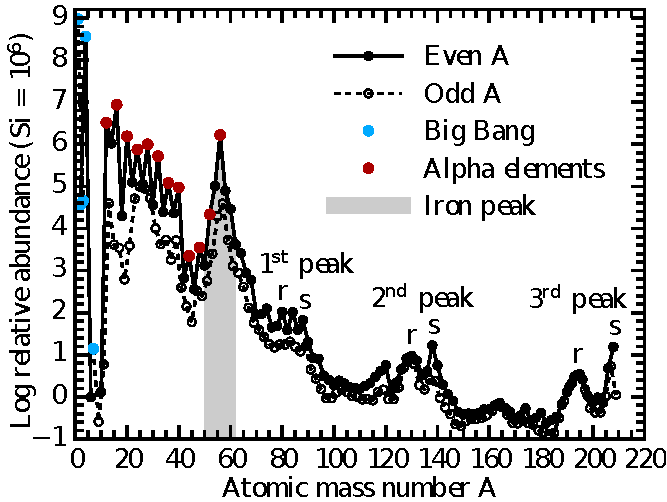
\includegraphics[width=0.49\textwidth]{Fig_1_1_Lip.pdf}
    \caption{Observed abundances in our solar system as a function of mass number
        $A$. The lightest elements were created in the Big Bang and fusion in stars predominantly
        creates alpha elements. The iron peak is made in core-collapse and type
        Ia \acp{SN}. Elements beyond the iron peak are synthesized by the slow ($s$) and
        rapid ($r$) neutron capture processes. These processes produce three distinct double
        peaks. Abundance data from \citet{Lodders:2003}. (Adapted from \citet{Lippuner:2018phd})
    }
    \label{fig:nuc:fig11_lip}
\end{figure}

%\begin{sidenote}
%    \textcolor{red}{Figure with solar observed abundances, showing $r$-elements and $s$-elements}
%    The observed obundacnes as a function of atomic mass number $A$ are shown in figure Fig. (XXX). 
%(data from \cite{Lodders:2003}). The plot shows nuclei that are more bound (due to spin pairing of nucleons 
%\cite{Moller:1993ed}), \textit{i.e,} those with an even $A$ number, are more abundant. The lowest binding 
%energy of nuclei with odd number of neutrons and protons (but even $A$) are largely unstable or short-lived. 
%A few exceptions are \textit{e.g.,} $^{40}$K, $^{50}$V, $^{138}$La and $^{176}$Lu, 
%that have a half-life of at least $10^{9}$ years.
%\end{sidenote}

The dominant \nuc{} process, responsible for the production of elements, varies with the mass 
number $A$.
%
For instance, light elements $A<8$ were synthesized right after the Big Bang
in the process known as \ac{BBN}.
Nuclides before the iron peak, $12\leq A\leq 56$ come from stellar hydrostatic 
nuclear burning \citep[\eg][]{Rolfs:1988,Hasen:2004}.
Elements at the iron peak $50\leq A \leq 62$ produces mostly 
during the type Ia \acp{SN} or explosive silicon burning in \acp{CCSN} \citep[\eg]{Woosley:2002}. 
The conditions at these sites are such that the dense material at the \ac{NSE}\footnote{
    At \ac{NSE} three parameters describe the composition: 
    density, temperature and electron fraction, $Y_e = n_p/(n_p + n_e)$, 
    where $n_e$ and $n_p$ are the (total) number density of electrons and protons 
    respectively \citep{Seitenzahl:2009}. 
    The composition at \ac{NSE} favors more tightly bound nuclides,
    as they are more difficult to photodissociate.
}, 
expands and cools down, enriching the \ac{ISM} with heavy elements \citep{Iwamoto:2000as}. 
%
%Most of the material beyond iron peak are produced via neutron capture processes 
%\citep{Burbidge:1957}.
Nuclides with $A\geq 56$ cannot be synthesized via standard cycles due to their 
strong Coulomb barriers. 
Thus, processes that do not involve charged particles become dominant. 
These are the neutron capture processes \citep{Burbidge:1957}.


%% -------------------------------------------------------
%%                   Nucleosynthesis Cites
%% -------------------------------------------------------

%\subsection{Nucleosynthesis up to the iron peak}
%
%
%\subsubsection{Big Bang nucleosynthesis}
%
%Light elements in the Universe, like hydrogen ($\sim 75\%$ by mass) and helium 
%($\sim 25\%$ by mass) alongside trace amounts of $^{3}$He and $^{7}$Li were created 
%during the \ac{BBN} (see \eg, \citet{Tytler:2000qf} and references therein). 
%And while only a small number of nuclides were involved in \ac{BBN}, 
%there are large discrepancies between \ac{BBN} models and observations. 
%For instance, the "lithium problem" \citep{Coc:2013eha}, which origin is not well 
%understood \citep{Fields:2011zzb}.
%
%
%\subsubsection{Low-mass stellar burning}
%
%In order to fuse massive nuclides and overcome the strong Coulomb barrier, high temperatures, 
%($\geq 10^6$ K) are required. Thus production of heavy elements from hydrogen and helium 
%is possible only in special environments, in particular, in the interior of stars 
%\citep{Bethe:1939}. 
%For the most of their lives stars burn hydrogen into helium. The process releases the 
%binding energy and maintains the hydrostatic stability of a star. After the hydrogen is 
%exhausted in the core, a core (atmosphere) contracts (expands), heats up (cools), and the 
%shell hydrogen burning is initiated, slowly depositing ashes, \eg, helium, into the inert core. 
%The star's subsequent evolution depends primarily on its mass. If the mass of a star 
%$M>0.5M_{\odot}$, at some point the helium in the core starts to fuse into $^{12}$C and 
%$^{16}$O and small amounts of $^{24}$Mg, $^{28}$Si. These elements are called 
%\textit{alpha elements} \citep{Rolfs:1988,Hasen:2004}. 
%The end of the core helium burning phase leads to another core contraction phase. 
%A star of a mass $\sim 8M_{\odot}$ would be able to ignite carbon and oxygen producing 
%heavier elements afterwards. A less massive star looses its outer layers and becomes a 
%slowly cooling degenerate core, a white dwarf.
%
%
%\subsubsection{nuclear burning is massive stars}
%
%For a star that has $M\geq 8M_{\odot}$, a sequence of burning stages follows, each of 
%which leads to the exhaustion of a respective fuel, contraction of the core and rise of 
%its temperature \citep{Woosley:2002}. Carbon burning leads to the production of 
%$^{20}$Ne, $^{23}$Na and free protons that contribute to the synthesis of non-alpha elements. 
%As temperature increases, the photodisintegration of $^{20}$Ne becomes possible and a small 
%amount of $^{24}$Mg is formed. Next, the oxygen burning occurs producing $^{28}$Si $^{31}$P, 
%and $^{28}$Si and $^{32}$S, that become dominant nuclides in the core by the end of oxygen burning \citep{Rolfs:1988}.
%
%The subsequent silicon burning proceeds at $T\sim3.5\times10^9$K through photodissociation 
%of some of the $^{28}$Si and a sequence of alpha particle captures, "alpha ladder", on the 
%remaining $^{28}$Si to form $^{32}$S, $^{36}$Ar, $^{40}$Ca, $^{44}$Ti, $^{48}$Cr, $^{52}$Fe 
%and $^{56}$Ni. This process lasts around a day \citep{Rolfs:1988,Hasen:2004}. Due to high 
%temperatures present at silicon burning, nuclides with $A\in[28, 62]$ fall into quasi-equilibrium, 
%meaning that these nuclides (with exception of $^{12}$C, $^{16}$O $^{20}$Ne and $^{24}$Mg), 
%alpha particles and protons participating in reactions, are in equilibrium with each other. 
%
%At $A=56$ the binding energy per nucleon appears reaches its maximum and the silicon burning 
%cannot produce heavier nuclides with the release of energy. As the fraction of $^{56}$Ni in the 
%core of a star increases, the support that nuclear burning has provided against gravitational 
%contraction falls. Meanwhile the mass of the degenerate core still increases as burning proceed in shells.
%However, when the electron degeneracy pressure can no longer counteract gravity, \ie, when mass 
%of the core exceeds the effective Chandrasekhar mass\footnote{
%    The collapse however occur before the core reaches Chandrasekhar mass, and the pressure 
%    support that rests on the availability of free electrons drops when electrons capture on 
%    the nuclides becomes possible. To account for this, the effective Chandrasekhar mass was 
%    introduced.
%}, 
%the core collapses leading to a \ac{CCSN} \citep{Woosley:2002}.
%Thus, the origin of more abundant alpha elements in the Universe is stellar fusion.
%
%
%\subsubsection{Iron Peak}
%
%At temperatures higher then $T\sim 5\times10^{9}$K nuclear \ac{NSE} establishes. This is a 
%balance between the fusion reactions forming a ($N,Z$) nuclide from $N$ neutrons and $Z$ 
%protons and photodissociation reactions, splitting it back. 
%At \ac{NSE} three parameters describe the composition: density, temperature and 
%electron fraction $Y_e = n_p/(n_p + n_e)$, where $n_e$ and $n_p$ are the (total) 
%number density of electrons and protons respectively \citep{Seitenzahl:2009}. 
%%
%The composition at \ac{NSE} favors more tightly bound nuclides, as they are more difficult 
%to photodissociate. Thus, if the conditions allow, \ie, temperature, density and electron 
%fraction of the mater, ($Y_e \sim 0.46$, an electron fraction of iron), nuclides at $A\sim56$, 
%\ie, iron peak elements, dominate \citep{Seitenzahl:2009}. 
%%
%For example, \ac{NSE} establishes during the type Ia \acp{SN}, when a thermonuclear 
%explosion of a white dwarf allows for sufficiently high temperatures and densities. 
%After the explosion, newly synthesized elements of the iron peak cools, and being stable, 
%remain in the expanding medium \citep{Iwamoto:2000as}.
%
%
%\subsection{Nucleosynthesis beyond the iron peak}
%
%Nuclides with $A\geq 56$ cannot be synthesized via standard cycles due to their strong Coulomb 
%barriers. Thus, processes that do not involve charged particles become dominant. 
%These are the neutron capture processes.
%%
As nuclides absorb neutrons and grow larger, their binding energy, $Q_n$, decreases. 
This process stops when $Q_n\sim1$~MeV and energetic photons start to knock out 
neutrons from a nucleus. This process is called photodisintegration and its location 
in the parameter space, (that in turn dependents on temperature and density), is called 
the 
%% [IMPORTANT]
neutron drip line 
%% ---
\citep{Rolfs:1988}.

Nuclides produced via neutron capture are generally unstable to $\beta$-decay, with a timescale, 
$\tau_{\beta}$, that can be larger or smaller than a neutron capture timescale, $\tau_n$. 
In case when $\tau_{\beta}\ll\tau_n$, \ie, when a $\beta$-decay occurs faster then the next 
neutron capture, the process is called \textit{slow} or \sproc{}. 
Thus, by definition, the \sproc{} moves along the valley of stability\footnote{
    a region of stable nuclides in the nuclides chart (a chart in terms of 
    number of neutrons $n_n$ 
    and number of protons $n_p$).
}, departing no further than by a few nuclides away.
On the other hand, if $\tau_{\beta}\gg\tau_n$, \ie, when a neutron capture occurs much 
faster then a $\beta$-decay, the process is called \textit{rapid} or \rproc{}. This \nuc{} 
generates nuclides near (but not crossing) the neutron drip line 
(See Fig.~\ref{fig:nuc:fig16_lip}) \citep{Rolfs:1988}. 

\begin{figure}[t]
    \centering
    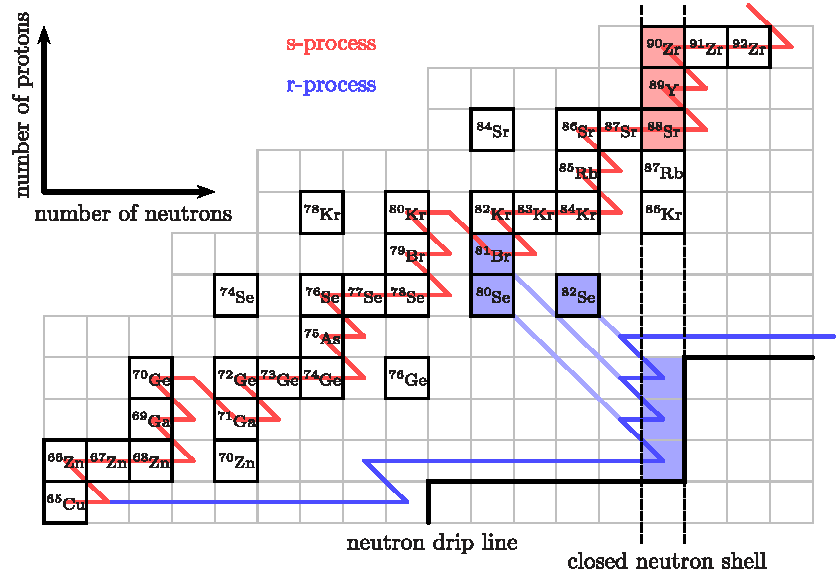
\includegraphics[width=0.60\textwidth]{Fig_1_6_Lip.pdf}
    \caption{Schematic representation of the $s$- and $r$-process on a section of the
        chart of nuclides. The \sproc{} (red) proceeds along the valley of stability and the
        \rproc{} (blue) along the neutron drip line. At the closed neutron shell $N = 50$, the
        neutron capture cross section drops by several orders of magnitude, which leads to a
        pile up of material there that produces the double-peak features
        (Adapted from \citet{Lippuner:2018phd})
    }
    \label{fig:nuc:fig16_lip}
\end{figure}

%% --- IMPORTANT --- ORIGIN OF THE PEAKS IN r-PROCESS
Notably, the trajectory of \rproc{} is interrupted when the neutrons within a nuclide can arrange 
themselves in a closed shell. Such configurations are energetically very favorable and thus the 
cross-section for a subsequent neutron capture reduces. Only after several $\beta$-decays does the 
\rproc{} continue. Thus, nuclides located at points where neutron drip line and a closed neutron 
shell overlap is more abundant. These unstable nuclides will decay back to the valley of stability 
and some of the neutrons within them turn to protons, reducing the total mass. The indication 
of this "overproduction" are the peaks in the abundance patterns at a mass, $A$, slightly lower then 
the one corresponding to a closed shell nuclide (see Fig.~\ref{fig:nuc:fig11_lip}).
%
%%% --- important
A similar "overproduction" of nuclides with a closed neutron shell occurs for the \sproc{}, 
%However, in that case it is caused by the cross section of these nuclides being 
%$1-2$ order of magnitude smaller then of neighboring ones \citep{Rolfs:1988}. Thus, in the case of 
%\sproc{}, 
but the peaks in abundance pattern will be at $A$, corresponding to the closed shell exactly, 
and thus located at larger $A$ than that of the \rproc{}. 
%
Closed shell nuclides are located at 
$N=50,\: 82, \: 126$ and thus corresponding abundance peaks for \sproc{} are at 
$A=88, \: 138, \: 208$ and at $A=80,\:130,\:194$ for \rproc{} (see \eg, \citet{Arnould:2007gh}) 
(See peak structure in Fig.~\ref{fig:nuc:fig11_lip}).

%% --- Motivation MP stars --- THE GENERIC SOLAR ABUNDANCES
%It was found, that the solar \rproc{} abundance pattern is general, and can be found anywhere in the 
%Universe: in stars that were formed very early on a galactic evolution timescale, \ac{MP} halo stars,
%that naively speaking, should not have had enough time to be formed out of material enriched by 
%\sproc{} and \rproc{} elements and show abundances similar to solar
%%For instance, in stars that were formed very early on a galactic evolution timescale, the 
%%\ac{MP} halo stars, one would expect to observe less \sproc{} and \rproc{} elements as there might have 
%%been not enough time for the enrichment to take place. However recent studies showed that the solar 
%%\rproc{} abundances are present in these stars as well 
%\citep{Sneden:2008,Roederer:2010}, 
%See also Fig.~$8$ in \citet{Sneden:2009}. 
%%Thus, modeling the \rproc{} \nuc{} it is expected to reproduce the solar abundances.

%%% -- can be deleted
%It is important to note that in addition to \sproc{} and \rproc{}, a possible $i$-process, (intermediate) 
%is widely discussed. The process operates further from the valley of stability than \sproc{}, but not 
%reaching neutron drip line \citep{Cowan:1977,Bertolli:2013gka}. Slow and intermediate neutron capture 
%processes operate within the low-mass \ac{AGB} stars with mass $M\in[1.5,3]M_{\odot}$ and more massive stars,
%that enrich the interstellar medium with heavy elements via strong winds 
%\citep[\eg][]{Peters:1968,Couch:1974,Kaeppeler:1994K,Woosley:2002,Straniero:2005hc,Herwig:2011}. 
%The possible cites for the \rproc{} we discuss in the following subsections.


\subsubsection{Possible $r$-process sites}

Study of possible cites of \rproc{} is a wide and rapidly developing field. The general requirement 
for \rproc{} is a low electron fraction, or, in other words, neutron-rich conditions. These can be 
found in various places for certain models of Big Bang, that include inhomogeneities, 
\ac{BNS} and \ac{NSBH} mergers and \ac{SN} ejecta (see \citet{Mathews:1990} and references therein). 
%
Spectral studies of \ac{MP} stars (formed early in the galactic history), combined with models of 
galactic chemical evolution sheds light on possible dominant cite of \rproc{} material. 
%\textcolor{red}{add more sources/models}. 
It is now believed that certain types of \acp{SN} and \ac{BNS} mergers are the most likely 
sources on \rproc{} material \citep{Mathews:1990,Thielemann:2011,Siegel:2019mlp} %\textcolor{red}{add more sources}


%\subsubsection*{\acp{CCSN}}

Collapse of a massive star produces a hot neutron core, that undergoes deleptonization, releasing 
$\sim10^{53}$~erg of binding energy in a form of strong neutrino flux. These neutrinos, irradiating 
dense medium around the core, can produce a \nwind{} \citep{Qian:1996xt}, that was suggested to be 
a promising cite for \rproc{} \citep{Woosley:2002,Wanajo:2006mq}. Later, it was shown however, that 
the electron fraction in the wind would be too high for a full \rproc{}, and only ``light'' heavy 
nuclide, up to $A\sim130$, can be synthesized 
\citep{Qian:1996xt,Thompson:2001ys,Fischer:2010,Roberts:2010,MartinezPinedo:2012rb,Wanajo:2013} 
%\textcolor{red}{add Perego:2017} 
%
%It is important to note that in the proton-rich \nwind{} nuclides with $A\sim 100$ can be produces 
%via so-called $\nu p$-process. The process relies on a creation of a free neutron from proton by 
%an antineutrino capture. These free neutrons can then be captured by a seed nuclide, $^{64}$Ge seed 
%nuclide and thus nuclides heavier then $^{64}$Ge can be created
%\citep{Frohlich:2006,Pruet:2005qd,Wanajo:2010mc,Arcones:2012}
%
A full \rproc{} can be achieved in so-called magnetorotationally driven \acp{CCSN}. 
This is a rare type of \acp{CCSN}, where a core of the progenitor is rotating rapidly 
and is strongly magnetized. Induced by a magnetorotational processes \eg, \ac{MRI}, 
collapse is accompanied by a formation of a collimated bipolar jet 
\citep{Wheeler:2000,Akiyama:2003,Burrows:2007yx,Mosta:2014jaa,Mosta:2015,Siegel:2019mlp}.
Materiel in these jets is predicted to be sufficiently neutron rich to allow for a full 
\rproc{} \nuc{} \citep{Winteler:2012,Nishimura:2015nca}. The rarity of this type of \acp{SN}, 
however, might not allow for them to be the dominant source or \rproc{} material 
\citep{Nishimura:2015nca} 

%Mergers of \acp{NS} we discuss separately in Sec.~\ref{sec:intro:bns_ejecta}

%\subsubsection{Compact object mergers}
%\red{TO BE REWRITTEN -- REPETITION OF PREVIOUS CHAPTERS}


%% --- MIGHT NEED TO BE SHORTENED A LOT!  OR MOVED TO INTRODUCTION!
Mergers of two \acp{NS} or a \ac{NS} and a \ac{BH} are regarded as one of the main cites 
of \rproc{} material (See Sec.~\ref{sec:intro:bns_merg}). 
%Compact objects, formed in a binary evolution of massive stars, 
%orbit each other for gigayears, before slow loss of energy from the system due to \acp{GW} 
%reduces their orbit and they merge \citep[\eg][]{Hulse:1975,Lattimer:2004sa,Price:2006fi}. 
%
%The late inspiral and merger of \ac{BNS} or a \ac{NSBH} have been studied extensively via smooth particle 
%simulations \red{[REFS]} \ac{HD} simulations \red{[REFS]} and \ac{NR} simulations with simplified gravity \red{[REFS]} 
%or full \ac{GR} \red{[REFS]}. The composition of a \acp{NS} in these simulations have been modeled with 
%simplified polytropic \red{[REFS]} or piece-wise polytropic \red{[REFS]} or microphsyical \acp{EOS} \red{[REFS]}. 
%The physical setup of these simulations have also evolved to eventually include effects of
%neutrino radiation transport \red{[REFS]} and magnetic fields \red{[REFS]}. 

%These studies have shown that shortly before and during the merger, the neutron star(s) undergo(s) a tidal 
%deformation and disruption. Streams of neutron-reach matter are then ejected into the circombinary 
%with enough energy to be not graviationally bound to the system \citep{Price:2006fi,Foucart:2014nda,Sekiguchi:2015dma,Kyutoku:2015gda,Radice:2016dwd}. 

%% For details on the ejecta from \ac{BNS} mergers see Chapter \ref{ch:BNS_results}.
%% In addition, in case of a \ac{BNS}, when \acp{NS} collide, material at the collision interface, heated by shocks, 
%% gets 'squeezed' and launched in the directions perpendicular to the plane of the binary \cite{Bauswein:2013,Hotokezaka:2013b} \red{[REFS]}. 
%% Generally, these tow components, tidal and shocked, constitute the \textit{dynamical ejecta}. Where the term 
%% ejecta referrers to the material that has enough energy to leave the system. 
%% The properties of the dynamical ejecta from BNS have a broad distribution, especailly in terms of mass and ejectron fraction 
%% [\red{[REFS]} \& myFitPaper], where the former lies in range $(10^{-4},10^{-2})M_{\odot}$ and the latter $(0.05,0.45)$. 
%% We discuss dynamical ejecta properties of BNS in more details in section \red{sec:results:dyn\_ej:prop} and nucleosynthesis 
%% in it in \red{sec:results:dyn\_ej:nucleo}. In case of NSBH the ejecta mass was shown be larger, reaching $0.1M_{\odot}$ with 
%% low electron fraction, $\leq0.2$ but it requires that masses of BH and NS are comparable and BH is rapidly spinning 
%% \cite{Foucart:2014nda}\red{[REFS]}. If the BH is much more massive then NS, the latter would be 'swallowed' with no ejecta \red{[REFS]}.
%% After the merger, there are expected to be additional ejecta. For general postmerger configuration consists of a remnant, massive neutron 
%% star (MNS) or a black hole sorrounded by a disk (torus) of bounded matter. In the first case,  a strong neutrino flux from cooling MNS and 
%% disk can drive an outflow in the direction, perpendicular to the plane of the binary, the so-called \nwind{} 
%% (see Figure 1 from \cite{Perego:2014fma}) \red{[REFS],Jujibayashi+20}. This ejecta is expected to occure on a timescales of 
%% $\sim100$ms postmerger, be not very neutron rich $Y_e\sim(0.2-0.45)$ due to neutrino irradiation and have a mass of 
%% $(10^{-4}-10^{-3})M_{\odot}$ \red{[REFS]}. 
%% The massive nutron star born in a merger exhibit dynamical oscillations \red{[REFS]}. The $m=1$ mode, so-called 
%% "one-armed spiral instability" especially can persisit on a $\sim100$ms powtmerger timescale and become a dominant mode 
%% \red{[REFS], MainPaper}. This oscillations can inject energy within the disk, where via angular momentum transport it leads 
%% to an outer part of the disk to become unbound. This ejecta, the \textit{\swind{}} was shown to occur in all cases where the MNS is present. 
%% It has high electron fraction and its mass depends on a lifetime of the remnant, and for a $\sim100$ms it can amount to a few 
%% $\times\sim10^{-2}M_{\odot}$ \red{[Letter, MainPaper]}. We discuss the mechanism that drives the \swind{} in the section 
%% \red{sec:results:swind:mechanism} and the ejecta properties in \red{sec:results:swind:prop} and corresponding 
%% nucleosynthesis in \red{sec:results:swind:nucleo}.
%% On a longer timescales, the viscous processes and alpha recombination in the disk, surrounding MNS or a BH are expected 
%% to unbind additional material. This is so-called \textit{secular ejecta}. It is expected to be massive and neutron rich. 
%% However, due to long timescales involved, it is very difficult model \red{[REFS]}.

\ac{BNS} and \ac{NSBH} mergers eject neutron rich material 
in which \rproc{} can take place, producing nuclides beyond $A=300$. Over-saturated with neutrons, 
nuclei are unsubtle to fission, and decay shortly after being formed. The decay products, 
before they reach the valley of stability, capture again free neutrons and grow up to 
$A=300$ and the cycle repeats. 
%% -- important 
This is so-called fission cycle. %\red{might be better to remove it from here and discuss later}
%\subsubsection{Fission cycling}
%Fission cycling is a process where freshly synthesized via strong \rproc{} heavy nuclides 
%with $A\sim 300$ undergo fission just to become seed nuclides for a similar \rproc{} 
%leading to an $A\sim 300$ nuclide. 
%This process eliminates the dependency of the final abundances on the initial conditions and 
%it also limits the maximum nuclide mass that can be achieved. 
%%
%The number of fission cycles can be estimated via a ration of the seed nuclides at time 
%zero and the number of seeds at the time when there are no more free neutrons available. 
%This is motivated by the fact that neutron capture itself does not create new seeds, only
%increases the mass of them, while fission, splitting heavy nuclide in two, generates 
%additional seeds. 
%%
%The number of fission cycles is tight to how much lanthanides and actinides are produced. 
%In particular, as fission cycling limits the maximum mass of the nuclide that can be created, 
%the fraction of lanthanides, actinides as well as heating $\varepsilon$ are insensitive 
%to the initial $Y_e$. The number of cycles is thus tight to the initial $Y_e$. The lower it is,
%the more free neutrons available and thus more cycles would occur. After the fission cycling
%stops the $r$-process maximum mass drops to $A\sim 250$. Thus the amount of actinides drops as
%only the lightest of them can be produced that do not fission immediately. 
%% --- 
It is maintained as long as there are free neutrons. After, the nuclides decay to the valley of 
stability for the last time, forming the remarkably robust abundance pattern, independent of the 
number of cycles \citep{Korobkin:2012uy,Bauswein:2013yna,Mendoza-Temis:2014mja}, 
(see also Figure 4 in \citet{Korobkin:2012uy}).
%
%Numerical models have shown that the final \rproc{} abundances in the \ac{BNS} and \ac{NSBH} 
%mergers ejecta are robust and reproduce the solar ones robustly 
%\citep{Freiburghaus:1999,Goriely:2011vg,Goriely:2015fqa,Wanajo:2014wha,Just:2014fka,Radice:2016dwd}\red{[Refs]}. 
%Recent observations of the one and only detected so far merger have confirmed that \ac{BNS} mergers do 
%produce \rproc{} elements \red{[Refs] incl. Stroncium paper}.


\subsubsection{Galactic chemical evolution}

While there are several generally accepted cites for the \rproc{}, the main one is yet to be 
determined \citep[\eg][]{Qian:2000bh,Argast:2003he,Matteucci:2014}
%
%%% DELAY
For instance, the observed \rproc{} enrichment of \ac{MP} stars 
%if \ac{BNS} mergers are the main cite, than 
%the observed \rproc{} enrichment is difficult to explain as it 
requires very early source of \rproc{} material, when no mergers 
should have had happened yet, as the inspiral time ads the time delay of order 
%This time delay before the compact binary binary formation and merger is 
$10^{6} - 10^{9}$ years \citep{DeDonder:2004cx,Dominik:2012kk}, and is highly uncertain and 
depends on a poorly understood common envelop evolution phase of the massive binary (progenitors)
\citep[\eg]{Dominik:2012kk}. 
%%%% SCATTER
Additionally, mergers of compact objects are rare events and thus expected to introduce 
a considerable scatter into the \rproc{} elements distribution in the Galaxy. 
However, observations show that the distribution is more uniform than expected \citep{Argast:2003he}.
%%%% CCSN as a contributor
Recent population synthesis models have indicated that with a contribution from 
magnetorotationallydriven \acp{CCSN} the compact object mergers can account for the 
observed scatter of heavy elements \citep{Ishimaru:2015,Cescutti:2015,Wehmeyer:2015,VanDeVoort:2015}.
%
%%%% --------------------------------
%%%% IN MORE  DETAILS 
%%%% --------------------------------
%%%% Delay
%After the \ac{BBN}, the Universe consisting of hydrogen and helium, with traces of lithium, have expanded and cooled. 
%Under the influence of dark matter, the primordial gas fragmented, clumped and first stars, galaxies and galaxy 
%clusters have formed. During their lifetime the first stars (population III stars) converted light elements into 
%heavier ones and then ejected them into the \ac{ISM} during \ac{SN} events. Future populations of stars were born 
%of gas enriched with heavy elements, in particular, iron. Thus, the amount of elements heavier then hydrogen and 
%helium is stars (\ie, metallicity) increased with each stellar generation and there exists an age-metallicity relation 
%\citep{Matteucci:2012}. Important to note, that multiple dark matter sub-halos contributed to the formation of the 
%galaxy and there might not be a unique age-metallicity relation (see \eg, \citet{Ishimaru:2015} and references therein).
%%% Delay
%The enrichment of interstellar medium with heavy elements from stellar interior occurs immediately after stars die. 
%However, the \rproc{} elements, produced in \ac{BNS} (\ac{NSBH}) mergers can only enrich \ac{ISM} when compact objects 
%inspiral and merge which on average takes $(0.1-1)\times10^{9}$ years \citep{DeDonder:2004cx,Dominik:2012kk}. 
%The exact delay time is however highly uncertain and depends on a poorly understood common envelop evolution phase of the binary 
%(progenitors). And it was shown, that a small percentage of compact binaries might form with a time delay 
%before merger as small as $10^{6}$ years \citep{Dominik:2012kk}. 
%
%%% Study observations
%To study the chemical evolution of stars in the galaxy, the spectroscopic surveys\footnote{
%    And indicative quantity of metallicity measured in such iron-to-hydrogen ration, [Fe/H], that reads as a $\log_{10}$
%    of the abundance of a element $X$ to hydrogen, normalized to solar ration, \ie, in the sun for every X, [X/H]$= 0$. 
%    If a stars has [Fe/H]$=-2$, it is said that this star ahs a 100 times less iron compared to hydrogen then sun.
%} are conducted \citep{Edvardsson:1993,Suda:2008na}. 
%%% Scatter
%Mergers of compact objects are rare events and thus expected to introduce a considerable 
%scatter into the \rproc{} elements distribution in the Galaxy. However, observations show that the 
%distribution is more uniform than expected \citep{Argast:2003he}.
%%% Scatter
%However, recent population synthesis models have indicated that with a contribution from 
%magnetorotationallydriven \acp{CCSN} the compact object mergers can account for the observed 
%scatter of heavy elements \citep{Ishimaru:2015,Cescutti:2015,Wehmeyer:2015,VanDeVoort:2015}.
%
%% 244Pu
Comparison between the solar system and earth crust abundances of $^{244}$Pu have indicated that this 
nuclide might have been produced in rare events with high yields \citep{Wallner:2015}. This statement 
was confirmed via models of galactic mixing \citep{Hotokezaka:2015zea}, that also showed that there 
appears to be no degeneracy between rare high yields events (\ac{BNS}/\ac{NSBH}) 
and frequent low yield ones (\ie, \ac{CCSN}). Similar conclusion was draws from studying $^{244}Pu$ 
abundances in meteorites \citep{Tsujimoto:2017}.
%
%% UFDG
Study of \acp{UFG} also point towards a rare high yield events for \rproc{} \nuc{}. In particular, 
the \ac{UFG} Reticulum II was shown to have a solar \rproc{} abundances, while \ac{UFG} of similar 
type tend to have $2-3$ times less \rproc{} elements. This suggests that a rare high-yield event 
has modified Reticulum II chemical composition and high europium abundances indicate that it was a 
compact object merger \citep{Ji:2016}. 
%
%Thus it is still unclear whether observed degree of homogeneity in \rproc{} elements distribution in the galaxy and 
%\rproc{} elements enrichment of very \ac{MP} stars can be explained by compact object mergers only. 
%% Scatter

%\red{Mention Actinide abundaces problem.}

%% --------------------------------------------------------------------------
%%               K I L O N O V A
%% --------------------------------------------------------------------------

\subsection{Kilonova}

Nuclides, synthesized in \rproc{} are very neutron rich and unstable. After the last 
fission cycle, they decay to the valley of stability.% (see chapter~\ref{ch:nucleo}). 
%
%This process takes from hours to days and released energy 
%can power an \ac{EM} transient, called \ac{kN} or Macronova  
%\citep[\eg][]{Li:1998bw,Kulkarni:2005jw,Metzger:2010,Roberts:2011,Metzger:2016pju,Wollaeger:2017ahm}
%
%
%During the \ac{BNS} mergers, the neutron-rich material is ejected 
%(see Chapter \ref{ch:bns_sims} for details). The conditions of the eject are such that they allow 
%for the \rproc{}, that produces heavy elements far from the valley of stability (see Chapter 
%\ref{ch:nucleo} for details) 
Li et al., \citep{Li:1998bw} suggested that an \ac{EM} transient can be powered by 
the radioactive decay of the material enriched with \rproc{} elements, ejected in 
\ac{BNS} or \ac{NSBH} mergers. They also showed that contrary to the normal \acp{SN}, 
the ejecta would quickly become transparent to its own emission, peaking on a timescale 
of around a few days. The main difficulty in this pioneering work was the lack of a \nuc{}
 model to model to estimate the radioactive heating of the ejecta. 
%
The understanding of \ac{kN} has significantly improved since then
\citep[\eg][]{Kulkarni:2005jw,Metzger:2010,Roberts:2011,Metzger:2016pju,Wollaeger:2017ahm}
%
but the only unambiguous detection of \ac{kN} so far, was the thermal transient, \AT{}, 
\citep{Coulter:2017wya,Chornock:2017sdf,Nicholl:2017ahq,Cowperthwaite:2017dyu,Tanvir:2017pws,Tanaka:2017qxj}
that was observed after the \ac{GW} trigger, \GW{}, 
\citep{TheLIGOScientific:2017qsa,Abbott:2018wiz,LIGOScientific:2018mvr}.
%
This observation provided evidences that the ejection of neutron-rich matter from compact 
binary mergers is one of the primary site for \rproc{} nucleosynthesis 
%\citep{Lattimer:1974slx,Li:1998bw,Kulkarni:2005jw,Rosswog:2005su,Metzger:2010,Roberts:2011,Kasen:2013xka}.
\citep{Arcavi:2017xiz,Coulter:2017wya,Drout:2017ijr,Evans:2017mmy,Hallinan:2017woc,Kasliwal:2017ngb,
    Nicholl:2017ahq,Smartt:2017fuw,Soares-santos:2017lru,Tanvir:2017pws,
    Troja:2017nqp,Mooley:2018dlz,Ruan:2017bha,Lyman:2018qjg}. 
%The \ac{kN} is the \ac{EM} \ac{UV}/optical/\ac{NIR} transient, powered by the 
%radioactive decay of the elements synthesized via \rproc{} in expanding ejecta.
%
The peak in \ac{NIR} band of \AT{} occurred several days after the merger \citep{Chornock:2017sdf}.
It is generally consistent with emission from the high opacity material, with a sizable 
fraction of lanthanides \citep{Kasen:2013xka}
%
The peak in \ac{UV}/optical band, however, occurred in less than one day after the merger 
\citep{Nicholl:2017ahq}. This requires the opacity of the material to be sufficiently low, 
suggesting that only partial \rproc{} \nuc{} took place in the corresponding ejecta 
\citep{Martin:2015hxa}.
%
These observations that material with distinctly different properties contributed to the emission.
%
% [RED]
%\ac{kN} has a complex observational signature due to different ejecta components with various 
%compositions contribution to it. 
In particular, it was shown that if produced, 
lanthanides $(58\leq Z \leq71)$ and actinides $(90\leq Z \leq 103)$ with their open 
$f$-shell and hence a plethora of absorption lines, increase opacity of emitting 
region by a factor of $10$. 
%
These elements are produced only if electron fraction of the ejecta was sufficiently low, 
$Y_e\leq 0.25$ \citep{Lippuner:2015gwa}, present for example in a tidal component of \ac{DE}. 
High opacity would imply that a transient is dim $(\sim10^{40})$ erg s$^{-1}$ and peak around a 
weak after merger in the red/infrared band \citep{Barnes:2013wka,Grossman:2013lqa,Lippuner:2015gwa}. 
%
% [BLUE]
If the ejecta electron fraction is high, $Y_e \geq 0.25$, weak \rproc{} would produce a small amount 
of lanthanides and the opacity of the emitting region would thus be lower. The kilonova signal originating 
from such ejecta would be bright and peak on a timescale of a few days in blue band 
\citep{Kasen:2014toa,Martin:2015hxa}. 
%
%
Indeed, both and red components were observed in the case of \AT{}, that confirmed the general 
picture \citep[\eg][]{Villar:2017wcc}. However, estimated mass of the ejecta required to explain 
the red component is larger then what is predicted by numerical relativity simulations \red{refs}. 
It is believed that the most contribution to this component comes from the low $Y_e$, slow but 
massive outflow from the degenrate disk on a secular timescale \red{refs}.
%
Semi-analytic two-components (red and blue) spherical \ac{kN} models to the \AT{} observations 
provided estimates for the ejecta properties for these two components. 
%
Specifically, for the langhinide poor (rich) \ie, blue (red) components, the required mass is 
$2.5\times10^{-2}M_{\odot}$ ($5.0\times10^{-2}M_{\odot}$) and velocity $0.27$c ($0.15$c)
\citep{Cowperthwaite:2017dyu,Villar:2017wcc}. 
See however \citep{Waxman:2017sqv} for an alternative interpretation.
See also \citep{Siegel:2019mlp} for the compiled data on the \ac{kN} models.
%
Similar estimates are obtained with $1$D radiation transport \ac{kN} models
\citep{Tanvir:2017pws,Tanaka:2017qxj}.
%
%A very high energy emission from the non-thermalized radiation is weak and can be 
%detected only for a sufficiently close event \cite{Hotokezaka:2015cma}.
% 
Notably, prior to \AT{}, there were other candidates based on the detection of \ac{SGRB}, 
with infrared excess \eg, 
GRB130603B, \citep{Berger:2013wna,Tanvir:2013pia}, 
GRB060614 \citep{Jin:2015txa,Yang:2015pha}, 
GRB050709 \citep{Jin:2016pnm}.
GRB200522A \citep{WRONG}  Bruni:2021ilp
However the exact nature of the observed signals were not well constrained. 
%
The search for \ac{EM} counterparts to mergers continues, involving observatories around the world 
\citep{Law:2009,Singer:2014qca,Bellm:2014,Kasliwal:2016uhu}.

%% --------------------------------------------------------------------------
%%               A F T E R G L O W S
%% --------------------------------------------------------------------------

\subsection{$\gamma$-ray bursts and kilonova afterglows}

\acp{GRB} are irregular pulses of gamma-ray radiation with broken power-law 
(non-thermal) spectrum, peaking at KeV-MeV \citep{Band:1993,Kouveliotou:1993,Meegan:1992xg}.
%
With respect to the duration, \ac{GRB} are split into two categories: \ac{SGRB}, 
that last ${\leq}2$~s and long \ac{GRB} that last ${\gtrsim}2$~s. The latter are the 
result of the collapse of massive ${\geq}15M_{\odot}$ stars, while the former, at 
least in part, is attributed to mergers of compact objects. Only very recently it 
was directly confirmed with the detection of \ac{SGRB} \GRB{} that accompanied 
the \ac{GW} event \GW{} \citep{TheLIGOScientific:2017qsa}. However, the exact physical 
origin of different duration \ac{GRB} is not fully understood.
%
Indications that long \ac{GRB} are associated with core-collapse supernovae, \acp{SN}, 
are two fold. These \acp{GRB} are typically observed in star-forming regions of their 
host galaxies \citep[\eg][]{Bloom:2000pq,Bloom:2002hc,Fruchter:2006py,Christensen:2004yx,CastroCeron:2006jh} 
and several \acp{GRB} are spectroscopically associated with Type Ic \acp{SN}, albeit 
these \acp{GRB} were significantly less bright and might not be typical \acp{GRB} 
\citep[\eg][]{Liang:2006ci,Bromberg:2011fm}. Additionally, the late time behaviour 
of some \acp{GRB} includes a \acp{SN}-like "bump" in the optical and spectral changes 
that might imply that underlying \acp{SN} flux becomes dominant over \acp{GRB} 
\citep[\eg][]{Bloom:1999,Woosley:2006fn}.
%
The \acp{GRB} are distant events, most of which were localized to outside the local 
group \citep[\eg][]{Mao:1992,Piran:1992,Fenimore:1993}. Particularly useful for distance 
estimation were the observations of \ac{GRB} afterglow, fading X-ray \& optical emission, 
that allow to estimate the redshift \citep[\eg][]{Costa:1997cg,Frontera:1997ae}.
%
Analysis of the multi-wavelength afterglow data for \acp{GRB} \citep[\eg][]{Panaitescu:2001bx} 
suggested the mechanism behind the afterglow emission is the synchrotron radiation from the 
external forward-shock, which forms when \ac{GRB}-ejecta sweeps-up the \ac{CBM} or \ac{ISM}
medium\footnote{
    The specific indications are the power law decay of the light curves, 
    $F_{\nu}\propto^{-1}$ and power-law spectrum $F_{\nu}\propto\nu^{-0.9\pm 0.5}$.
} 
\citep{Rees:1992ek,Paczynski:1993gz,Meszaros:1993ju,Meszaros:1996sv}.
%
The temporal behavior of many (but not all) \acp{GRB} shows a change, a steepening 
of the light-curve (to $F_{\nu}\propto t^{-2.2}$) at $\sim 1$~day after the burst. 
This is usually attributed to the 
%\gray{deceleration of the colimated GRB-outflow, jet, and decrease on the realtivisitc beaming. This in turn makes the edge of the jet visible to an observer.} 
finite angular extend of the \ac{GRB}-ejecta, jet \citep[\eg][]{Rhoads:1999wm,Sari:1999mr}. 
When jet decelerates and relativistic beaming decreases (and the jet edge becomes visible), 
the optical and X-ray lightcurves decay achromatically faster. This achromatic transition 
from slow to faster decay is called "jet-break".
%
%%% PROBLEMO -- jet-break is not a universal feature.
%Notably, this jet-break is not observed in all \acp{GRB} for the reason that is not fully 
%understood \citep[\eg][]{Fan:2006pj,Panaitescu:2006,Liang:2007ti,Sato:2006jg,Liang:2007rn,Curran:2007cp,Racusin:2008bx}
%%
%%% PROBLEMO -- GRB density seems uniform, but SSE models predict wind-like profile
%Models of the broadband emission of \acp{GRB} with jet-break showed that the 
%\ac{CBM}, is uniform with number density \red{$\sim 10^{-3}$} \citep{Panaitescu:2001bx}. 
%If \acp{GRB} produced in collapse of massive stars \citep{Woosley:1993,Paczynski:1997yg}, 
%this contradicts the expected density profile from stellar winds, \eg, $\rho\propto r^{-2}$ 
%\citep[\eg][]{Dai:1998iz,Chevalier:1999jy,Chevalier:1999mi,Ramirez-Ruiz:2001} 
%\red{this might be very outdated.}
%
%% sGRB
The origin of \acp{SGRB} was first connected with the elliptical galaxes, and with 
older stellar population 
\citep[\eg][]{Gehrels:2005qk,Fox:2005kv,Barthelmy:2005bx,Berger:2005dr,Panaitescu:2005er,Bloom:2005qx,Guetta:2005bb,Nakar:2007yr} 
and thus with \ac{BNS} mergers. A more direct evidence came with the \GRB{}
\citep{Savchenko:2017ffs,Alexander:2017aly,Troja:2017nqp,Monitor:2017mdv,Nynka:2018vup,Hajela:2019mjy}, 
detected by the space observatories Fermi \citep{TheFermi-LAT:2015kwa} and INTEGRAL \citep{Winkler:2011}.
%
Generally \acp{SGRB} show a complex time behavior of early afterglow X-ray emission, 
in particular a presence of a plateau ($F_{x}\propto t^{-1/2}$), after the initial sharp 
decrease ($F_{x}\propto t^{-3}$) which a standard forward shock model does not predict. 
This implies that early X-ray afterglow is shaped by a variety of physical processes 
\citep{Zhang:2005fa}.
%
The \GRB{} was dimmer then any other events of its class. 
Different interpretations for its dimness and slow rising flux were proposed: off-axis jet, 
cocoon or structured jet. Now it is commonly accepted that \GRB{} was a structured jet 
observed off-axis 
\citep[\eg][]{Fong:2017ekk,Troja:2017nqp,Margutti:2018xqd,Lamb:2017ych,Lamb:2018ohw,Ryan:2019fhz,Alexander:2018dcl,Mooley:2018dlz,Ghirlanda:2018uyx}.
The \GRB{} late emission, the afterglow, provided information on 
the energetics of the event and on the properties of the circumburst medium 
\citep[\eg][]{Hajela:2019mjy}. 

%%%% EARLY emission problem
%Two main questions stem from these observations: is the mechanism behind the prompt 
%$\gamma$-ray emission and early afterglow emission is the same (or do they originate from 
%the same outflow), and is the early X-ray radiation produced by the external shock (just a 
%blast wave takes long time to become self-similar) or does it originate from an internal 
%shock? An indication that the long-lived central engine activity might affect the 
%afterglow came from the observed sharp increase in X-ray flux (flares) on a 
%scale of minutes to hours after the end of the \ac{GRB}
%\citep{Burrows:2005ww,Chincarini:2007fp,Chincarini:2010,Margutti:2011}, 
%which could not be attributed to the inhomogeneities in the \ac{CBM}.
%%% PROBLEMO!
%Thus, the early X-ray behaviour of \acp{GRB} $t < 10^{4}$~s post-burst is not well 
%understood and seems to be in tension with standard afterglow forward shock emission model.

%\textcolor{red}{
%    One of the foremost unanswered questions about GRBs is the physical mechanism
%    by which prompt $\gamma$-rays the radiation that triggers detectors on board
%    GRB satellites are produced. Is the mechanism the popular internal shock
%    model 6 \cite{(Rees and Meszaros, 1994)}, the external shock model, or something
%    entirely different? Are $\gamma$-ray photons generated via the synchrotron process
%    or inverse-Compton process, or by a different mechanism? Answers to these
%    questions will help us address some of the most important unsolved problems
%    in GRBs  how is the explosion powered in these bursts? Does the relativistic
%    jet produced in these explosions consist of ordinary baryonic matter, electron positron
%    pairs, or is the energy primarily in magnetic fields?
%}

%Once again, while it is suggested that the high energy emission, after the propmt phase is produced 
%by the synchrotron process in the external forward shock, \citep{Kumar:2009,Ghisellini:2010}, 
%the mechanism behind the high and low energy $\gamma$-ray emission in the prompt phase remains unknown. 
%Possible mechanisms include: inverse Compton and synchrotron emission in internal and external shocks
%\citep[\eg][]{Rees:1992ek,Dermer:1998py,Lyutikov:2003ih,Zhang:2011} and 
%photospheric radiation with contribution from multiple \ac{IC} scatterings
%\citep[\eg][]{Thompson:1994zh,Ghisellini:1998jy,Meszaros:1999gb,Peer:2005qoc,Peer:2008udu,Giannios:2006jb,Ioka:2007qk,Asano:2009gi,Lazzati:2010,Beloborodov:2010,Toma:2011}.

%% from the Afterglow paper



%\subsection{kilonova afterglow}

In addition to the \ac{GRB} beamed emission, the non-thermal, more isotropic 
emission is expected from electrons accelerated in shocks formed between the 
(mildly) relativistic ejecta and the \ac{ISM} \citep{Nakar:2011cw}. This emission 
is expected to peak in radio band and continue on a time scale of tens of years 
after merger. Notably, all ejecta components will contribute to the emission, 
but depending on the ejecta velocities and kinetic energy, 
the brightness in different frequencies and timescales differs. 
%
Various ejecta components interact with each other and with \ac{ISM}. The latter, 
generates a long-lived blast wave. The shock, propagating upstream, amplifies 
(random) magnetic fields and accelerates electrons, that subsequently emit 
synchrotron radiation. This process in phenomenological similar to the for the 
\ac{GRB} afterglow and \ac{SN} early remnants. 
%
Numerical simulations of \ac{BNS} mergers showed the presence of mildly relativistic 
ejecta (See Sec.~\ref{sec:bns_sims:method:ejecta}). 
Several studies on the possible non-thermal electromagnetic emission of this ejecta 
have been carried out 
\citep[\eg][]{Piran:2012wd,Hotokezaka:2015eja,Hotokezaka:2018gmo,Radice:2018pdn}. 
Notably, the observed non-thermal emission from \GW{}, was first interpreted 
as the non-thermal emission from the ejecta \citep{Mooley:2017enz}.
This interpretation was however disproved by the emergence of jet break
%
%Specifically, a strong radio emission is expected from \ac{BNS} ejecta \citep{Piran:2012wd,Hotokezaka:2015eja}. 
The \ac{BNS} merger radio remnant is expected to peak on a time-scale 
of years after the merger and be visible over a similar timescale. Notably, this is 
assuming that the ejecta is expanding into the unshocked \ac{ISM}, as it was shown 
that if the \ac{ISM} is pre-shocked by the jetted outflow, and the \ac{ISM} density is 
reduced, the kilonova afterglow would be delayed. 
%
In \citet{Piran:2012wd}, the synthetic \ac{kN} afterglow \acp{LC} are calculated 
for a set of \ac{NR} \ac{BNS} merger simulation with properties typical to the 
Galactic binary population and \ac{ISM} density usually found in the Galactic disk, 
$\nism\sim1\ccm$. Authors showed that the from a binary of two $1.4\Msun$ \acp{NS}, 
the kilonova afterglow would peak $\sim10$~years after the merger if $\nism = 0.1\ccm$ 
and $\sim3$~years if $\nism = 1\ccm$ in radio bands, $\nu=1.4$~GGz and $\nu=150$~MGz. 
Notably, both values of the \ac{ISM} density are larger than what is inferred for \GW{}. 
Indeed, jet fitting models and dependent analysis of the diffuse emission suggest 
$\nism\in(10^{-4},10^{-2})$\gcm \citep{Hajela:2019mjy}.
%In \citet{Piran:2012wd} authors focus on the observational prospects of this afterglow 
%and compare it to other \ac{EM} emission expected for \ac{BNS}. 

%% =====================================================================================
%%
%%              T H E O R E T I C A L  P I C 
%%
%% =====================================================================================

\section{Theoretical picture of \ac{BNS} mergers}

In This section we briefly overview the current understanding of the \ac{BNS} 
merger, the dynamics of the inspiral, effects of tides, \pmerg{} hydrodynamics 
and open questions.

%% --------------------------------------------------------------------------
%%               I N S P I R A L
%% --------------------------------------------------------------------------

\subsection{Inspiral}

If \acp{NS} formed through a classical stellar evolution channel of the massive binary, 
their orbit is mostly circular with little to non eccentricity \cite{Aasi:2013wya}. 
%
The binary system looses energy to the emission of \acp{GW}, and the orbit of \acp{NS} 
shrinks. Stars inspiral. The last ${\sim}10^3$ orbits, for instance, can be completed in 
a matter of minutes. During the last part of the inspiral, the \ac{GW} signal rises in 
frequency and amplitude (so-called chirp), reaching the peak at \textit{moment of merger}.


\subsubsection{Two Body Dynamics}

The dynamics of two well separated stars that have relatively small angular velocity 
(\ie, quasi-adiabatic inspiral of point-masses) the \ac{PN} approximation to \ac{GR}, 
(the expansion in $\upsilon/c$, with $\upsilon/c\ll 1$) is applicable.
%In other words, this is the stage of evolution when the orbital timescale is 
%significantly larger than the orbital one, \ie, $\dot{\Omega}/\omega^2\ll 1$.
%
The amplitude and the phase evolution of the \ac{GW} signal, at the leading order, 
is given by the quadruple formula 
%
\begin{equation}
\label{eq:intro:gw_wave}
h(t) \sim \frac{1}{d}\mathcal{M}_c^{5/3} f_{GW}^{2/3} = \nu\frac{M}{d}(Mf_{GW}(t))^{2/3}, \hspace{5mm} \phi(t) \sim 2\mathcal{M}_c^{-5/8}t^{5/8} = 2\nu^{-3/8}(t/M)^{5/8},
\end{equation}
%
where $\mathcal{M}_c = M\nu^{3/5}$ is the chirp mass, $M = M_A + M_B$ is the binary mass, 
$\nu = M_A M_B/M^2$ is the symmetric \mr{}, $f_{GW} = \dot{\phi}$, $d$ is the distance of the source.
%Here, the $G=c=1$ are the units, and geometric coefficients are neglected for brevity.
%
Obviously, \acp{NS} are not point-masses. The \ac{NS} finite size affects (tidal effects) the 
inspiral and, consequently, emitted \acp{GW}. In the \ac{PN} formalism these effects enter 
and $5$th \ac{PN} order.
%
%The \ac{PN} expansion, being the asymptomatic expansion, looses its accuracy at high 
%frequencies $f_{GW}\gtrsim 50\,$Hz. 
%
Another approximation to the two-body dynamics in \ac{GR} is the \ac{EOB} formalism,
which is a Hamiltonian formalism, applicable to all stages of the binary evolution.
%It is has an advantage of being applicable both at low and high frequencies and can be 
%applied throughout the inspiral, merger na \pmerg{} \cite{28}.
It spiritually similar to that, commonly used in Newtonian dynamics to 
describe the motion of two bodies via the motion of a single particle with effective mass 
$\mu=\nu M$ in the effective potential. Approximating the dynamics in \ac{GR} requires 
employing effective particle, $\mu$ and defective metric. 
%
Damour \& Nagar \cite{Damour:2009wj} extended the \ac{EOB} formalism to \ac{BNS} mergers by 
introducing finite size effects. For the up-to-date review we refer tp \cite{Damour:2012mv}.


\subsubsection{Effects of tides}

A method to treat the finite-size effects in self-gravitating objects in \ac{PN} 
dynamics was, proposed by Damour, Soffel and Xu \cite{Damour:1983a}, is based on ``skeletonizing'' 
objects into worldlines with global properties -- the \textit{outer problem}.
%
It was matched to the \textit{inner problem}, that considered how the worldtube 
around one body is influenced by another. In the case of \ac{BNS}, the latter is 
referred to the tidal effects induced by the external gravitional field of the companion. 
%Matching the outer problem with the inner translates into the inclusion of the tidal 
%deformation effects into the orbital dynamics (and consequently, \ac{GW} emission). 
The fully relativistic formulation of the \textit{inner problem} was derived in 
\cite{Hinderer:2007mb,Damour:2009vw,Binnington:2009bb}. 
%The key parameters of the formulation are the 
%external tidal moments,
%introduced as symmetric-trace-free projections of the derivatives of the externally 
%generated parts of the local gravitoelectric, $\bar{E}_{\alpha}$ and gravitomagnetic, 
%$\bar{B}_{\alpha}$, fields that read 
%$G_L^A = \partial_{\langle L-1}\bar{E}^A_{\alpha_l\rangle}|_{X^{\alpha}}\rightarrow 0$, 
%(where $X^{\alpha}$ are local coordinates \cite{32}).
%In the local frame of the first body, the \red{internally generated mass} $M_L ^A$ and spin 
%$S_L ^A$ multipole moments, (here $L=i_1,i_2,...,i_l$, is the multi-index) depend on the external
%tidal moments via 
%\textit{tidal polarizability coefficients} $\mu_l$ and $\sigma_l$, expressed as 
%
%\begin{equation}
%    M_{L}^{A} = \mu_l G_{L}^A, \hspace{5mm} S_{L}^A = \sigma_l H_L^A,
%\end{equation}
%
%where $M_L ^A$ and $S_L ^A$ are the internally generated mass and spin miltipole moments.
%(here $L=i_1,i_2,...,i_l$, is the multi-index), and 
%$G_{L}^A$ and $ H_L^A$ are the external tidal moments, related to gravitoelectric and 
%gravitomagnetic fields respectively. 
The key components of the formulation are the external gravitoelectric 
(gravitomagnetic) fields, $l$-th order of which induces the mass (spin) multipolar moments 
of the same order in \ac{NS}. These moments are characterized by %$G\mu_l$ ($G\sigma_l$), 
tidal polarizability coefficients, that can be written as dimensionless relativistic 
Love numbers \cite{Damour:2009vw,Binnington:2009bb}.
%
%The $l$-th order (external) gravitoelectric (gravitomagnetic) fields induce $l$-th order 
%mass (spin) multipolar moments in a \ac{NS}, characterized by respective coefficients, 
%$G\mu_l$ ($G\sigma_l$), that have dimensions of [length]$^{2l+1}$.
%%
%The dimensionless relativistic Love numbers are defined as
%%
%\begin{equation}
%k_l = \frac{(2l - 1)!!}{2}\frac{G\mu_l}{R^{2l + 1}}, \hspace{5mm} j_l = \frac{(2l-1)!!}{2}\frac{G\sigma_l}{R^{2l+1}},
%\end{equation}
%
%where $R$ is the radius of a \ac{NS}. 
%In many studies, only the dominant $l=2$ mode is considered, \eg, \cite{33}. 
%For \acp{BH}, $\mu_l=\sigma_l=0$ \cite{32,34}.
%Sometimes, only dominant quadrupole $l=2$ gravitoeletric coeffcient is considered \cite{33}.
%
If the external field can be viewed as quasi-static (``adiabatic tides'') the 
Love numbers can be computed by considering the stationary perturbations of the spherical 
relativistic star, \ie, solving the \ac{TOV} equations, which are considered in full \ac{GR}, 
due to strong dependency of the tidal coefficients on the star compactness, defined as 
$C_{i} = GM_i/R_i^2c^2$. 
%
Thus, Love numbers carry the imprint of the \ac{EOS} on the \ac{BNS} dynamics.
%
%On the other hand, if the external field is dynamic, than the effects induced by a \ac{NS}, 
%at linear order in the deformation, can be formulated as a superposition of the proper modes 
%of the \ac{NS}. The excitation of modes occur when the resonant frequency of modes is matched 
%by the star's orbital frequency. 
%This approach has been studied in Newtonian gravity, in \ac{GR} for a test-mass circling the 
%\ac{NS}, and for \acp{NS} of similar mass in \ac{PN} theory \cite{35,36,37}.
%Dynamical external field induces ``dynamical tides'', among which the most important are the 
%pressure modes ($f$-modes) in the non-resonant way\footnote{
%    The resonance for $f$-modes occur in kHz
%    regime, that is achieved only at merger, when two \acp{NN} are no longer isolated objects. 
%    Other mode,s such as $g$- and $r$-modes do not contribute significantly, due to their 
%    lower energies (albeit also lower frequencies).
%}
%
%The tidal effects can be included into the \ac{PN} two-body dynamics by modifying the 
%\ac{GR} effective action as 
%%
%\begin{equation}
%S = S_{GR} + S_{pointmass} = \frac{1}{16\pi G}\int R\sqrt{|g|}dx - \sum_{A}\int M_A \dd s_A
%\end{equation}
%%
%where the last term of the \ac{RHS} is the ``skeletonized'' representation \red{as} a point mass, 
%with non-minimal coupling of worldlines, that read 
%%
%\begin{equation}
%S_{nonminimal} = \sum_{A}\frac{\mu_l^{A}}{2l!}\int (G_L^A)^2 \dd s_A + \frac{l \sigma_l^A}{l! 2(l+1)} \int(H_{L}^A)^2 \dd s_A.
%\end{equation}
%%
%The added term changes the dyanmics at $5$th \ac{PN} order. The change is linear in tidal deformations.
%%
%At the leading \ac{PN} (Newtonian) order, only $l=2$ gravitoelectric terms appear when tidal 
%contributions are included. The term reads 
%%
%\begin{equation}
%\label{eq:intro:tidal_largangian}
%L^{LO}_{tidal} = k_2^A G M_B^2\frac{R_A^5}{r^6} + (A\leftrightarrow B),
%\end{equation}
%%
%where $r$ is the distance between \acp{NS}. 
%
Writing the modified \ac{GR} action with the inclusion of ``skeletonized'' representation
of a \ac{NS}, the tidal effects can be added into the \ac{PN} description of the two-body dynamics.
The resulted Lagrangian, at the leading (Newtonian), order shows that at small distances 
between stars, $r$, the introduced corrections are attractive. 
%
Further, the Kepler law given by the quadrupolar gravitoelectric term, 
%
%\begin{eqnarray}
%\Omega^2 r^3 = G M \Big[ 1 + 12 \frac{M_A}{M_B} \frac{R_A^5}{r^5} k_2^A + (A\leftrightarrow B) \Big].
%\end{eqnarray}
%
shows that the finite-size effects manifests as an increased orbital frequency at a given radius.
In other words, the \acp{NS} spin faster, if tidal effects are present and merger sooner 
producing signal with higher frequency \cite{Damour:2009wj}. 
%When $r=R_A+R_B$, the frequency at merger can be estimated. 
%There, $2GM\Omega\approxeq2(M_B/(MC_B) + M_B/(MC_B))^{-3/2}$ \cite{29}. 
%For \acp{NS} of the same mass one obtains 
%%
%\begin{equation}
%f_{GW}^{contact} \approxeq 1.327 \Big( \frac{C}{0.15} \Big)^{3/2} \Big( \frac{M}{2.8M_{\odot}} \Big) \text{kHz}.
%\end{equation}
%
%Simulations show that the contact between the two \acp{NS} happens approximately 2-4 \ac{GW} cycles 
%prior to merger at an even lower frequency \cite{38}

Within the \ac{EOB} framework, the dynamics of the system can be expressed in terms of the 
effective Hamiltonian, $H_{EOB}$
%that for zero-spin case can be written 
%%
%\begin{equation}
%H_{EOB} = M\sqrt{1 + 2\nu (\hat{H}_{eff} - 1)}, 
%\hat{H}_{eff} = \frac{H_{eff}}{\mu} = \sqrt{A(u;\nu)(1 + p_{\phi}^2u^2 + 2\nu(4-3\nu)u^2p_{r^*}^4) + p_{r^*}^2}
%\end{equation}
%%
%where $u=GM/rc^2$ is the Newtonian potential. 
%Consder the Schwarszchild spacetime and a particle in it with $\nu\rightarrow0$ and 
%$A(u;0) = 1-2u$. Then, the $H_{eff}$ becomes the particle Hamiltonian.
%
.
The finite-size effects can be included as tidal component to the potential, $A$, as 
$A = A_0 + A_{tidal}$ \cite{Bini:2012gu}, 
%that can be written as 
%%
%\begin{equation}
%A_{tidal} = \sum_{l\geq 2}\Big[ k_l^{A+}u^{2l+2}(1+\alpha_1^{(l+)}u ... ) + k_{l}^{A-}u^{2l+3}(1+\alpha_1^{(l-1)}u + ...) + (A\leftrightarrow B) \Big]
%\end{equation}
%%
%where $\alpha_i^{(l)}(\nu)$ are coefficients and 
%%
%\begin{equation}
%k_{l}^{A+} = 2k_l^A\big( \frac{M_A}{MC_A} \big)^{2l+1}\frac{M_B}{M_A}, \hspace{5mm} k_l^{A-} = 2j_l^A\Big( \frac{M_A}{M C_A} \Big)^{2l + 1} \frac{M_B}{M_A}
%\end{equation}
%%
%are the multipolar tidal polarizability coupling constants. 
that depends on the multipolar tidal polarizability coupling constants $k_{l}^{A\pm}$.
%
In the Newtonian limit the \ac{EOB} Hamiltonian reads 
%
\begin{equation}
H_{EOB} \approxeq Mc^2 + \frac{\mu}{2}p^2 + \frac{\mu}{2}(A-1) = Mc^2 + \frac{\mu}{2}p^2 + \frac{\mu}{2}\Big( -\frac{2 G M}{c^2 r^2} + \cdots - \frac{\kappa_2^T}{r^5} \Big).
\end{equation}
%
where $\kappa_2^T = \kappa_2^A + \kappa_2^B$ is the constant accounting for the tidal 
interactions at leading order.
%
For a physically motivated range of masses (1-2)$\Msun$ and \mr{}s $q\in[1,2]$ the 
$\kappa_2^T\sim[50,500]$. 
%
Similarly, one can defile the $\Lambda_2^i = 2/3 k_2^i (c^2 R_i/GM_i)^5$ with $i\in\{A,B\}$.
Then, instead of $\kappa_2^T$, the \textit{reduced tidal deformability} is used
%
\begin{equation}
\label{eq:theory:Lambda}
\tilde{\Lambda} = \frac{16}{13}\frac{(M_A + 12M_B)M_A^4}{M^5}\Lambda_A + (A\leftrightarrow B).
\end{equation}
%

Consequently, the effects of tides appear in the waveform computation, as radiation reaction 
compliments the conservative dynamics discussed above \cite{Damour:2008gu} and discussed in \cite{Damour:2012yf,Banihashemi:2018xfb}.
%
%At leading order the stationary phase approximation of the waveform reads
%%
%\begin{equation}
%h(f) = Af^{-7/6}e^{-i(\Psi_0(x) + \Psi_{tidal}(x))} = Af^{-7/6}e^{-i(\Psi_0(x)-39/4\kappa_2^Tx^{5/2})}
%\end{equation}
%%
%where $x(f) = (\pi G M f / c^3)^{2/3}$ and $\Psi_0(x)$ is point-mass phase.
%
Notably, the $k_2^T$ fully determines the tidal contribution to the waveforms at leading order. 
Hence, from observed \ac{GW} signal, the $k_2^T$ (or $\tilde{\Lambda}$) can be well estimated. 
%
%There have been extensive tests of the \ac{EOB} formalism for \ac{BNS} mergers agains \ac{NR} 
%simulations \cite{43,38,44,45,46}. 
%The accuracy of the \ac{EOB} approximation of tides, the $A_{tidal}$, decreases during 
%the last orbits and for very large $k_2^T$. Modified versions of \ac{EOB} were developed 
%with gravitational self-force calculations of tides computed at high-order TEOBResumS 
%\cite{44,47,46,48} and dynamical tides (SEOBNRT) \cite{49}.
%When spin cannot be neglected, the tidal interactions become more complex \cite{50,51}.
%The oblateness of a spinning \ac{NS} leads to the deformed gravitational field that is 
%characterized by the quadrupole tensor, and produces an attractive contribution to the 
%potential, modifying the inspiral at the $2$nd \ac{PN} order $\mathcal{O}(\upsilon/c)^4$
%\cite{50}. 
%There are also hybrid models of \ac{EOB} and \ac{NR} \cite{52,53}

\subsubsection{Gravitational Waves}

The most accurate way to compute waveforms is the conduct \ac{NR} simulations with microphysical 
\ac{EOS}. However, these simulations are computationally expensive and not avaiilable or feasible 
in certain renages of the parameter space.
The \ac{EOB} approach allows to compute the waveforms at broad range of frequencies and 
covers all stages of the binary evolution. 
The \ac{EOB} models can be augmented with the formulism descibing the 
high frequency emission of the remnant (kiloHertz), that itself can be build from the 
available \ac{NR} \ac{HD} simulations \cite{Bernuzzi:2015rla,Chatziioannou:2017ixj,Easter:2018pqy}.

From the \ac{GW} signal observed with ground based facilities, contains the information 
about the chirp mass, 
%(related to $I_{-10}$),
%where $I_p = \int \dd\ln f(\gamma(f))f x^{2p}(f)$ with $\gamma(f)df$ being the 
%measure of the detector noise \cite{59,6},
primarily at low frequencies. Additionally, the low frequency part of the signal, 
$\leq50$~Hz and $\leq100$~Hz contains information on the symmetric \mr{} and \ac{SNR}.
On the other hand, the information about tidal effects (tidal parameters) is related to 
%$I_{+10}$,
higher frequency signal, evaluation of which requires accurate high-frequency waveforms.
%
From the Newtonian limit discussed above, it follows that the system dynamics at merger 
is determined mainly by $\kappa_2^T$ \cite{Bernuzzi:2014owa}. \ac{NR} simulations verified this 
prediction \cite{Zappa:2017xba,Breschi:2019srl}. 

With respect to the \GW{} most of the information was obtained in $30-600$~Hz frequency 
range ($\sim 1300$ orbits).
The signal was interpreted as coming from a \ac{BNS} merger with total mass of $\simeq2.7\Msun$,
chirp mass $\mathcal{M}=1.186(1)\Msun$, \mr{} $q\in[1,1.34]$ and $\tilde{\Lambda}\simeq 300$ 
(with an upper bound of $\sim800$) \cite{TheLIGOScientific:2017qsa,Abbott:2018wiz,LIGOScientific:2018mvr}.
Inclusion of the \ac{EM} counterparts into the analysis leads to higher $\tilde{\Lambda}$ being 
more favoured \cite{Radice:2017lry,Radice:2018ozg}.
%
The estimation of individual masses and \mr{} was more subjected to uncertanties and 
systematic, \ie, spin prior \cite{2}. Due to the partial degeneracy between the tidal 
parameters and the \mr{}, the \ac{EOS} constraints are also subjected to uncertainties. 
Specifically, assuming that stars had small spin $\leq 0.05$, the stars radii can be 
constrained to $11-12$~km \cite{De:2018uhw,Abbott:2018exr}. 
Assuming also that \ac{EOS} can support a non-rotating \ac{NS} with a mass $1.97\Msun$, 
results in  $R\sim 11.9\pm 1.4$~km and $90\%$ credibility \cite{Abbott:2018exr}.
%
%\ac{GW} signal during the inspiral (including tidal phasing) also provides constraints 
%on the \ac{EOS} viewed in the pressure-density diagram \cite{65}. 
%For an example case of a \ac{BNS} with $\rho_{\rm max} \approxeq 2 \rho_0$, 
%the estimated value of pressure is $P(2\rho_0)=3.5_{-1.7}^{2.7}\times10^{34}$ dyn cm$^{-2}$ 
%at $90\%$ confidence level.
%
%For \GW{} the peak of the \ac{GW} signal, the merger, was not detected. However, from the 
%probability distribution of $\tilde{\Lambda}$, adopting \ac{NR}-motivated fitting 
%formula, it is possible to asses the peak frequency that falls in $1.2 - 2$kHz \cite{55}.
%The \ac{GW} peak luminocity is estimated to be $\geq 0.1\times 10^{56}$ erg/s \cite{61}. 


%% --------------------------------------------------------------------------
%%               P O S T - M E R G E R
%% --------------------------------------------------------------------------

\subsection{Merger and \pmerg{}}

After the \acp{NS} inspiral and merge, the dynamics of the system becomes significantly 
more complex, as temperatures and densities rise by orders of magnitude and new 
physical effects, \eg, magnetic fields and weak interaction, start to affect the evolution. 
The \pmerg{} phase is not well understood, and mainly explored with miltiphsyics \ac{NR} 
simulations with various degrees of sophistication and resolution. 

The summary of the \ac{BNS} \pmerg{} evolution is shown in Fig.~\ref{fig:RadFig1}. 
There are several trajectories that system can take, depending when the formed remnant 
collapses to a \ac{BH}. The early \pmerg{} phase is charaterized by strong \ac{GW} 
emission and hydrodynamic effects. After it, several interlinked processes guvern the 
evolution: the \ac{MHD} stresses, contributing to the angular momentum and redistribution 
and neutrino emission, that alters the matter composition and cools is.
If \ac{BH} does not form, the \ac{MHD} torques and residual \ac{GW} emission spin down 
the remnant.

\subsubsection{Dynamics and Thermodynamics Conditions}

Prior to the merger, the \ac{NS} can be considered as being in cold, neutrinoless, 
weak equilibrium with only marginal heating due to tidal deformation at the last orbits.
The dynamics at merger is dominated by the \acp{NS} orbital motion
as $\upsilon_{rad}\ll\upsilon_{orb}$\footnote{
    Orbital speed can be written as $\upsilon_{orb}\eqsim\Omega r\eqsim\sqrt{GM/(R_A + R_B)}$
    that for equal mass binary is $\upsilon_{orb}/c\eqsim\sqrt{C}\eqsim0.39(C/0.15)^{1/2}$.
    The radial velocity is beven by the evolution of the orbital frequency, as 
    $\omega_r \eqsim 2\Omega r \dot{\Omega}/(3\Omega^2)$. The $\dot{\Omega}$ can be 
    estimated from the fact, that orbital frequency satisfies 
    $\dot{\Omega}_{GW}\sim(3456/125)(G\mathcal{M}/c^3)^5\Omega_{GW}^{11}$ during the 
    inspiral. Then, the radial velocity reads 
    \begin{equation}
    \upsilon_r/c\eqsim\frac{192\pi}{15}\frac{G^3 M^3}{c^5(R_A + R_B)^3}\frac{q}{(1+q)^2}
    \end{equation}
    that for equal mass gives $\upsilon_r/c \eqsim 0.0034 (C/0.15)^3$.
}.
%Merger time, $t_{merg}$, estimated from the \ac{GW} frequency at \acp{NS} collisition 
%for comparable \ac{NS} masses is given by 
%\begin{equation}
%    t_{merg}\eqsim\frac{1}{2f_{GW}^{contact}}\eqsim1.50\text{ms}\Big(\frac{M}{2.8\,\Msun}\Big)^{1}
%\end{equation}
%where the frequency of \acp{GW} when \acp{NS} come into contact, \ie, when the distance 
%between them, $r = R_A + R_B$ can be evaluated from the Kepler law, given by 
%the quadrupolar gravitoelectric term, % Eq.~7
%$2GM\Omega \eqsim 2(M_B/(MC_B) + M_B/(MC_B))^{-3/2}$ \cite{29},
%as 
%\begin{equation}
%    f_{GW}^{contact} \eqsim 1.327 \Big(\frac{C}{0.15}\Big)^{3/2}\Big( \frac{M}{2.8\,\Msun} \Big) \text{ kHz}
%\end{equation}
that is $\upsilon_{orb}\eqsim\Omega r\eqsim\sqrt{GM/(R_A + R_B)}$, indicating that 
more compact binaries experience more rapid, more violent mergers.

% Remnant
When \acp{NS} collide, their deformed cores squeeze past each other, triggering \ac{KHI},
in the first bounce. After several of these bounces, the cores fuse into a single object.
At collision, \ac{KHI} is triggered by the \acp{NS} cores plunging into the companion,
squeezing past each other inducing first wave of gravity-driven compression. 
The maximum values of temperatures and densities are reached then \cite{Perego:2019adq}. As 
nuclear and centrifugal forces start to dominate, the cores bounce until gravity 
pulls them back. 
Notably, formed in the violent, fast collision, the remnant core while is being far from 
hydrodynamic equilibrium, does not exhibit shocks. This is due to high speed of sound 
of nuclear matter at supra-nuclear densities 
%($c_s\gtrsim0.2\, c$, at $\rho\gtrsim\rho_0$)
.
Shocks form at the \ac{NS} surface, accelerating matter to mildly-relativistic velocities 
(\ref{Sec:intro:bns:ejecta}).
Not processed by shocks, the fluid inside the cores remains cold 
%$T\lesssim10\,$MeV, $s\lesssim1\,k_B$/baryon 
throughout the merger. The fluid at the interface between bouncing cores, however,
heats up through compression and shear dissipation 
up to $T\sim70-110\,$MeV, creating a pair of hot regions, offset by $\sim\pi/2$ with 
respect to dense cold regions \cite{Kastaun:2016yaf}.
%
The evolution proceeds towards more axisymmetric, stable remnant, but can be 
interrupted by the \ac{BH} formation. 

%% Disk Foramtion
The matter outside the bouncing cores, lifted by tidal torques and squeezed at the 
collisional interface forms a disk (or a torus).
Due to different contributions with different properties, the disk is highly non-uniform.
The overall properties of the disk, such as mass, have complex dependency on 
binary parameters, that can be expressed, as a first approximation, via fitting 
formulae to \ac{NR} simulations \cite{Radice:2017lry,Radice:2018xqa,Radice:2018ozg}. 
As outer part of this quasi-adiabatically expands 
%with $T^3/\rho^3\sim\text{const}$ as the \ac{EOS} is dominated by non-relativisitc baryons
its inner region cools. 
%
As was mentioned above, the newly born remnant is not hydrodynamically stable. 
Its dynamics is characterized by the pronounced $m=2$ bar- and $m=1$ one-armed-
deformations \cite{}, \red{more}, inducing spiral waves, propagating through the 
disk \red{FIG}. Additionally, the former leads to the strong \ac{GW} emission 
in $\sim10-20$~ms \pmerg{}. The backreaction from the energy and angular momentum 
loss dumps the $m=2$ mode efficiently and \ac{GW} emission subsides. 
%We refer to this evolutionary phase as \ac{GW}-dominated \pmerg{} phase.
%Notably, the $m=1$ mode, however, can persist due to mode coupling 
%\cite{Dietrich:2016phd}. 
That makes the end of the ``\ac{GW}-driven phase'' of \pmerg{} evolution. 

% Disk Settling down 
Weak processes and spiral density waves, shocking periodically the fluid, 
bring the disk to the configuration, that can be described by smooth 
temperature profile 
%from $\sim10\,$MeV at $\rho\eqsim10^{13}$\gcm to $\sim0.1\,$MeV at $\rho\eqsim10^4$\gcm
%with entropy $\in(3,10)$ $k_B$/baryon
and quasi-Keplerian orbit.
%
% IF BH forms
If the remnant collapses to a \ac{BH}, the densest part of the disk is 
accreted on the dynamical timescale, reducing the total mass by half 
%and the disk maxiumum density to $\sim10^{12}\,$\gcm,
and radial extend \cite{Perego:2019adq}.

% Magnetic fields
While \acp{MF} are not expected to affect the \ac{BNS} inspiral, their influence 
on the postmerger evolution can be strong \cite{Duez:2006qe,Kiuchi:2017zzg}, as they get amplified 
to the values exceeding that of magnetar, $10^{16}\,$Gauss, by a range of processes, 
\eg, flux freezing and compression, \ac{KHI} at the collisional interface \cite{Kiuchi:2015sga},
\ac{MRI}, \cite{Duez:2006qe,Kiuchi:2017zzg} and \ac{MF} winding \cite{Duez:2006qe},
%

Whether the ordered, large-scale \acp{MF} can form in \pmerg{} environment 
via the dynamo process is presently unknown. The are important in producing 
polar collimated outflows, jets \cite{Bucciantini:2011kx,Ruiz:2016rai} and mildly relativistic outflows
\cite{Metzger:2018qfl,Fernandez:2018kax}. Random magnetic fields are also relevant for \pmerg{} evolution, 
as they generate stresses, enhancing angular momentum transport. Presently, 
these processes are not well understood, as seed \ac{MHD} instabilities operate at 
small scales (centimeters) and cannot be resolved in global \ac{MHD} \ac{BNS} merger 
simulations
% with reslistic initial condiitons.
One possibility, is enhance the seed \acp{MF} to bring the instabilities to larger 
scales \cite{Kiuchi:2015sga,Kiuchi:2017zzg}.

The effect of \acp{MF} on the angular momentum transport can be approximated via 
the $\alpha$-viscosity model \cite{Shakura:1972te}. These effects are important 
in detetrmining the remnant structure, lifetime and hence, the \pmerg{} \acp{GW} 
\cite{Radice:2017zta,Shibata:2017xht}. 
%The timescale for the angular momentum redistribution in the remnant \cite{80} 
%\begin{equation}
%    t_{rem} \eqsim \alpha^{-1}R_{rem}^2\Omega_{rem}c_s^{-2}\eqsim 0.56\,s\Big(\frac{\alpha}{0.001}\Big)^{-1}\Big(\frac{R_{rem}}{15\,\text{km}}\Big)^2 \Big( \frac{\Omega_{rem}}{10^4\,\text{kHz}} \Big) \Big(\frac{c_s}{0.2\,c}\Big)^{-2}
%\end{equation}
%where $\Omega_{rem}$ and $c_s$ are the angular momentum and sound speed respectively.
an the loss of angular momentum bring the remnant closer to either stable, 
rigidly rotating configuration of collapse \cite{Hotokezaka:2013iia}. 
%
The \acp{MF} effects within the Keplerian disk facilitate accretion \cite{Fernandez:2015use,Fujibayashi:2017puw,Fernandez:2018kax,Miller:2019dpt},
%on a timescale
%\begin{equation}
%    t_{disk} = \alpha^{-1}\Big(\frac{H}{R}\Big)^{-2}\Omega^{-1}_K \eqsim 0.78 \Big(\frac{\alpha}{0.02}\Big)^{-1}\Big(\frac{H/R}{1/3}\Big)^{-2}\Big(\frac{M_{rem}}{2.5\,\Msun}\Big)^{-1/2}\Big(\frac{R_{disk}}{100\,\text{km}}\Big)^{3/2}
%\end{equation}
%where $M_{rem}$ is the mass of the central remnant and $R_{disk}$ is the radial 
%scale of the disk.

%%%% Neutrinos
The prime cooling mechanism of the post-\ac{GW}-dominated phase is the emission of 
neutirinos, produced by hot, dense part of the disk and remnant, and that are 
able to escape \cite{Eichler:1989ve,Rosswog:2003rv,Sekiguchi:2011zd}. 
%The typical neutrino mean free path is 
%\begin{equation}
%    \lambda_{\nu} = \Big(n_B\sigma_0(E_{\nu}/m_e c^2)^2\Big)^{-1}\simeq 24.6\,\text{m}\,(\rho/10^{14}\,\text{g}\,\text{cm}^{-3})^{-1}(E_{\nu}/10\,\text{MeV})^{-2},
%\end{equation}
%where $n_B$ is the density of baryons, and 
%\begin{equation}
%    \sigma_0 \simeq 4G_{F}^2 (m_e c^2)^2 / (\pi(\hbar c)^4)\simeq 1.76\times 10^{-44} \, \text{cm}^2
%\end{equation}
%is the typical neutrino cross section scale, and $E_{\nu}$ is the neutrino energy.
%Considering the charactersitic remnant temperature as  $T_{rem}\simeq20\,$MeV 
%energy of the thermal neutrinos then $E_{\nu}\simeq 3.15T_{rem}$ and optical depth 
%$\tau_{\nu}\simeq R_{rem}/\lambda_{\nu}=\mathcal{O}(10^{4})$.
The neutrinos are radiated on a diffusion timescale \cite{Perego:2014fma}:
%\begin{equation}
%    t_{diff} \simeq \frac{\tau_{\nu}R_{rem}}{c}\simeq 4.28\,s\Big( \frac{R_{rem}}{15\,\text{km}} \Big)^{-1}\Big(\frac{M_{rem}}{2.5\,\Msun}\Big)\Big(\frac{T_{rem}}{20\,\text{MeV}}\Big)^2.
%\end{equation}

Within the remnant, neutrinos are in weak and thermal equilibrium with matter.
due to charged current reaction. There, production of $\nu_e$ is suppressed by 
degeneracy and as $\mu_n-\mu_p+\mu_e<0$ at high temperatures, the electron 
anti-neutrinos, $\bar{\nu}_{e}$, dominate. The effect of these ``trapped'' 
neutrinos on the remnant evolution is not very strong \cite{Foucart:2015gaa,Perego:2019adq}.
%
Within the disk, however, the optical depth for neutrinos is ${\simeq}1$ so 
the they can diffuse out on a timescale of milliseconds, lowering the disk 
temperature. The cooling rate is controlled by the degeneracy state of neutrinos 
%that is kept at mild values by the feedback negative effect, higher 
%values have on the cooling rate.
\cite{Beloborodov:2008nx}.

During the early \pmerg{}, the $L_{\bar{\nu}_e}\gtrsim L_{\nu_e}$, as the 
free neutrinos are abundant in the diskand the absorption opacity for $\nu_e$ 
exceeds that of $\bar{\nu}_e$.
Thus, alongside heating and decompression, the initially cold matter in weak 
equilibrium, undergoes \textit{leptonization} 
%The heavy neutrinos, $\nu_{\mu,\tau}$, are balanced by pair processes and 
%decouple from matter at higher densities and temperatures within the remnant
%namely $\rho\gtrsim10^{13}$\gcm and $T\gtrsim8\,$MeV 
\cite{Perego:2014fma,Endrizzi:2019trv}
%The, BNS simulations including
%neutrino transport predict the mean neutrino energies at infinity
%$E_{\nu_{e}}(\sim 10\,\text{MeV})\lesssim E_{\bar{\nu}_e}(\sim 15\,\text{MeV}) \lesssim E_{\nu_{\mu,\tau}}(\sim 20\,\text{MeV})$. Notably, binaries with higher mass 
%show higher neutrino energies \cite{14,86}.

Neutrinos with different energies decouple from matter in different regions.
%due to the stron dependency of the cross section on the incoming neutrino energy.
Average energy $\nu_{e}$ and $\bar{\nu}_e$ decouple at ${\sim}10^{11}$\gcm, found 
in the disk, while low energy neutrinos decouple at higher $\rho\sim10^{13}$\gcm.
The geometric surface along which neutrinos decouple is generally called ``neutrino 
surface'' \cite{Perego:2014fma,Endrizzi:2019trv}.
%The dependency of the location and the geometry of this surface on the thermodynamics 
%conditions and neutrino energy facilitates the need to coherent treatment of the 
%strong and weak interactions over a broad span of densities and temepratures.
Thus, the energy dependent (spectral) neutrino radiation trasport is required in 
\ac{BNS} merger simulations

While it has been shown that neutrino flavor conversions may occur in the \ac{BNS} 
\pmerg{} environment, \eg, the matter-neutrino oscillations, induced by the 
the fact that $\bar{\nu}_e$ decouple at smaller radii then $\nu_{e}$ \citep[\eg][]{Zhu:2016mwa,Tian:2017xbr}, 
and fast-flavor conversions above the neutrino surface \cite{Wu:2017drk}, their impact 
on the properties of the ejected material remains largely unexplored.
%More works of neutrino quantum kinetics equations \cite{90,91}, that include 
%collisional integral and angular and energy distributions of neutrinos are required.

One of the main unknowns with respect to \ac{BNS} mergers, is the high density part, 
$\rho{\gtrsim}\rho_0$ of the \ac{NS} \ac{EOS} \citep[\eg][]{Hebeler:2013nza,Oertel:2016bki}, that relate to the 
relevant thermodynamic degrees of freedom and nucleonic interactions. For instance, 
the emergence of the new species, \eg, hyperons, pions, muons, and nuclear 
resonances, would lower the matter degeneracy, and thus, soften the \ac{EOS} \citep[\eg][]{Fore:2019wib,Vidana:2010ip}.
Additionally, the emergence of to deconfined quark matter, due to \ac{QCD} phase transition,
would alter \ac{EOS} at very high temperatures and densities that not well constrained 
\cite{Busza:2018rrf}.


\subsubsection{Fate of the Remnant}

The end product of \ac{BNS} merger depends primarely on the binary parameters, (masses, 
\mr{}) and \ac{EOS}, and in particular, on the maximum supported mass of a non-rotating 
\ac{NS}, $M_{max}^{TOV}$ \cite{Shibata:2016}, as well as on the finite temperature and 
non-beta-equalibrium composition effects. 

The \ac{BH} formation directly at merger is usually referred to as \ac{PC}. 
The conditions for it depend on \ac{EOS} and not well understood. 
Simulations show that in equal mass binaries, \ac{PC} occurs if the total mass 
$M\gtrsim M_{thr} = k_{thr}M_{max}^{TOV}$, where $k_thr\in(1.3,1.7)$ that depends on 
\ac{EOS} \cite{Shibata:2005ss,Shibata:2006nm,Hotokezaka:2011dh,Bauswein:2013jpa}.
%(or $\kappa_2^T\lesssim43-73$, or $\tilde{\Lambda}\lesssim338-386$.
Simulations of uneqal mass binaries show that the threshold is lower \cite{Bauswein:2017vtn}, and 
$k_{thr}\propto C_{1.6}$, with $C_{1.6}$ being the compactness of the $1.6\,\Msun$ 
\ac{NS} \cite{Hotokezaka:2011dh,Bauswein:2013jpa,Bauswein:2017vtn}. As \ac{PC} cases are not expected to ejecta large 
amount of material and be \ac{EM}-loud (in case of comparable mass binary), the \GW{} 
is believed to be not a \ac{PC} case, \cite{Margalit:2017dij,Bauswein:2017vtn}. 

The remnant that does not undergo \ac{PC} is a massive \ac{NS}, temprarly suppoerted 
by fast rotation \cite{Baumgarte:1999cq, Rosswog:2001fh, Shibata:2005ss, Shibata:2006nm, Sekiguchi:2011zd, Hotokezaka:2013iia, Bernuzzi:2015opx}, whose lifetime depends 
intricately on the \ac{EOS}, finite temperature effects, and viscosity. A commonly 
adopted classification, based on the properties of equilibrium models (neglecting the 
dynamical and finite temperature, and magnetic effects), \ie, $M_{max}^{TOV}$ and
$M_{max}^{RNS}$\footnote{
    $M_{max}^{RNS}$ is the maximum mass of a rigidly rotating \ac{NS} (no differential 
    rotation) supported by zero-temperature (cold) \ac{EOS}. Also sometimes referred as 
    mass-shedding limit.
    % $M_{max}^{TOV}$ and $M_{max}^{RNS}$ are agnostic to thermal or magnetic eects 
    %which can impact the stability of the remnant in nontrivial ways (108, 72)
}
and include 
\ac{HMNS} if $M > M_{max}^{RNS}$, 
\ac{SMNS} if $M_{max}^{TOV} \leq M_{max}^{RNS}$,
and stable \ac{MNS} if $M < M_{max}^{TOV}$ \citep[\eg][]{Baumgarte:1999cq}.
The \ac{HMNS} is supported by differential rotation, that viscosity reduces with time. 
Hence, they are expected to collapse to a \ac{BH}. The \ac{SMNS} can avoid the collapse 
even after reaching rigidly rotating configuration. The lifetime of \ac{HMNS} and \ac{SMNS}
depends on efficiently of mass and angular momentum loss (to, \eg, massive winds) and 
finite temperature effects \cite{Radice:2018xqa}. Based on these uncertainties, we distinguish between
\textit{short-lived} remnants, that collapse to \ac{BH} during \ac{GW}-dominated phase, 
% taht correspods to ${\sim}10-20\,$ms after merger \cite{107,60}
and \textit{long-lived} otherwise.

If a remnant can achieve rigid rotation, its evolution then characterized by the emission 
of \acp{GW} (due to residual asphericity) and magnetic braking, reducing further its 
angular momentum, until either \ac{BH} forms, or stable non-rotating equilibrium is reached.
The observations of \acp{SGRB} with X-ray plateu \cite{Zhang:2000wx,Lasky:2015lej,Fan:2013cra}, if indeed given by the 
magnetar activity\footnote{
    There are other possible explanations behind the X-ray plateu emission of \acp{SGRB} 
    \cite{Oganesyan:2019jij}
}, suggest that the remnant may survive from seconds to hours \cite{Fan:2013cra, Ravi:2014gxa}.
Most of the energy, ${\sim}10^{52}\,$erg, that a remnant needs to lose before collapsing 
most likely is carried away in a form of \acp{GW}, as \ac{EM} observations of \GW{} suggest.
%This emission can be observed for the nearby event \cite{111}, priding direct information 
%on the remnant fate. However this emission was not observed for \GW{} \cite{67,68}

From \ac{EM} observations of the merger the fate of the remnant, albeit in the 
model-dependent way can be inferred. In case of \GW{}, the presence of such counterpart 
strongly disfavors \ac{PC} \cite{Margalit:2017dij,Bauswein:2017vtn,Radice:2017lry}, while leaving the question whether it was 
\ac{HMNS} or \ac{SMNS} open. Margalit \& Metzger \cite{Margalit:2017dij} suggested that the remnant 
was short-lived, on account of the non-detection of the expected ${\sim}10^{52}\,$erg, 
from the spin-down of the long-lived one. Assuming thus that \GW{} produced \ac{HMNS}, 
constraints can be placed on $M_{max}^{TOV}{\lesssim}2.2\Msun$ \cite{Margalit:2017dij}.

On the other hand, employing the magnetar model of \acp{SGRB} to \GW{} \cite{Ai:2018jtv,Li:2018hzy,Piro:2018bpl},
lead to the requirement of a very long-lived remnant (months) and weak dipol \acp{MF} \cite{Ai:2018jtv},
giving a different constraint on the maximum mass of the non-rotating star, 
$M_{max}^{TOV}{\gtrsim}2.2\Msun$ 
%and up to an order of magnitude lower ejecta mass ${\sim}10^{-3}\,\Msun$, that is attributed 
%to reducied amount of emergy from radioactive decay is required to explain the observed 
%UV/optical/infrared observations \cite{16}. 
%There have been indications of the X-ray flaring activity in \GRB{} \cite{117}, but 
%follow-up observations did not confirm it \cite{118}
. 


%% --------------------------------------------------------------------------
%%               M M  S I G N A T U R E S
%% --------------------------------------------------------------------------

\subsection{Multimessenger Signatures} % -> EM signatures

During and after the merger, neutron-rich material is ejected from the system on the 
dynamical \cite{Rosswog:1998hy, Hotokezaka:2013b, Bauswein:2013yna, Wanajo:2014wha, Radice:2018pdn} and secular \cite{Lee:2009, Perego:2014fma, Fernandez:2015use, Siegel:2017nub, Fujibayashi:2017puw, Fernandez:2018kax, Miller:2019dpt} 
timescales via a number of processes (see Sec.~\ref{sec:intro:bns:ejecta}), that 
undergo \rproc{} \nuc{}, synthesizing neutron-rich unstable elements \cite{Eichler:1989ve,Wanajo:2014wha,Cowan:2019pkx},
that subsequently decay, releasing energy that thermalizes and can be observed as 
an \ac{EM} transient, \ac{kN}, with quasi-thermal spectrum \cite{Metzger:2019zeh}. 

The non-thermal emission associated with \ac{BNS} mergers arise primarily from the
interaction between the fast ejecta and \ac{ISM} \cite{Kumar:2014upa,Piran:2012wd}. This include the 
\ac{kN} afterglow,
produced by aforementioned ejecta on a timescale of years and collimated 
relativistic outflow, jets, that are observed as bright flashes of high energy $\gamma$-rays, 
prompt emission, and late time afterglow across all \ac{EM} bands. \cite{Eichler:1989ve,Berger:2013jza} 
Notably, the origin of prompt emission is not yet fully understood \cite{Kumar:2014upa},
as well as the mechanism resposible for launching the jet. Several possibilities are 
considered in the literature. \gray{The \ac{BZ} mechanism, that extracts the rotational energy 
    from spinning \ac{BNH} in a strongly magnetized environment} \cite{Blandford:1977ds,Ruiz:2016rai}, magnetized winds 
from the remnant egulfed in strong \acp{MF} \cite{Zhang:2000wx,Bucciantini:2011kx} and neutrino-antineutrino powered 
fireballs \cite{Eichler:1989ve}.

Both, \ac{kN} and \ac{SGRB} were observed for \GW{}, called respectively, \AT{} and \GRB{} 
\cite{kilonova observation list}
\cite{grb observation list}
The $\gamma$-ray flash was detected $1.7\,$s after the \ac{GW} trigger by INTEGRAL and 
Fermi satellites \cite{Monitor:2017mdv}. The \GRB{} appeared dimmer than other transients of its class, 
which was attributed to the \ac{GRB} jet being a structured (not top-hat) jet with central axis
misaligned with the line-of-sight and the 
\cite{Lazzati:2017zsj,Xie:2018vya}\cite{Refs of a struct jet model}

%% Neutrinos
%\ac{BNS} mergers are expected to be strong neutrino emitters, on par with \acp{CCSN}, if 
%the remnant suvives sufficiently long for trapped neutrinos to escape \cite{72}. However, 
%detection of this emission is limited to the events in our galaxy, where the merger rate is 
%once every $\mathcal{O}(10^4)\,$years.
%The IceCube and VERITAS facilities can detect GeV/TeV neutrinos and photons that might originate 
%in \ac{SGRB} jet or in the remnant magnetosphere \cite{130,131} if the source is up to 
%${\sim}10\,$Mpc away. The origin of this very high energy emission, however, is not fully 
%understood, and their detection would be a ``new messenger'' from \ac{BNS} mergers.

%% postmerger GWs
%A large amount of energy ${\lesssim}0.1\,\Msun\eqsim 2\times 10^{53}\,$erg is radiated 
%over the ${\sim}10-20\,$ms after merger in a form of kHz \acp{GW} \cite{107, 60}.
%While this emission is below the sensitivity of current generation facilities 
%\cite{97,132,80,133}, it bay be observed by $3$rd gen detectors for close enough events 
%\cite{57}. 
%The main peak of \pmerg{} \ac{GW} signal, $f_2$, \cite{132,133,134,135} was shown to 
%correlate with $R_{1.6}$ \cite{132,80}, (and not with \ac{NS} spin and \mr{} \cite{134,135}).
%A more tight constraints can be obtained on the $\kappa_2^T$ (or $\tilde{\Lambda}$) from 
%$f_2$ via the quasi-universal realtion \cite{80,56,57,58,136} 

%% Phase transition and GWs
%Notably, the \pmerg{} observations of $f_2$, that itself is set by the orbital frequency 
%that depends on the $k_2^T$ allows to constrain the low-density physics (fixing the $R_{1.6}$ 
%and $k_2^T$) \cite{44}. Thus, $f_2$, is almost independent on the merger remnant star 
%deformations (until the collapse), as the rate of angular momentum loss is correlate with the rate of binding energy loss to \acp{GW} \cite{56,107,135,20}. 
%This trend was also snown to be robust with the presence of the $2$nd order phase transition 
%after merger, that allows for na additional energy release and amplification of \acp{GW} signal 
%\cite{9}. This is not exactly the case if the $1$st order phase transition is present, that 
%leads to the remnant contraction on the dynamical timescale and instead of angular 
%velocity, it is angular momentum that is conserved, \cite{11}.
%This such a phase transition can be undetified as disagreement between the $k_2^T$ obtained 
%from the inspiral \acp{GW} and \pmerg{} \acp{GW} \cite{11} (assuming \ac{PC} did not 
%occur\cite{10}).


\subsubsection{Mass Ejection, Kilonovae, and Nucleosynthesis}

\ac{BNS} mergers result in ejection of material that can can be observed, providing the 
information of the merger dynamics and properties of the binary, and enrich the 
\ac{ISM} with heavy \rproc{} elements \cite{Shibata:2019wef}. The quasi-thermal emission associated with 
the decay of heavy \rproc{} elements is qusi-isotropic and thus have higher changes to be 
observed \cite{Metzger:2019zeh}

The $\rproc{}$ \nuc{} in ejecta is primarily determined by the electron fraction \cite{Lippuner:2015gwa}, $Y_e$, 
producing $3$rd ($1$st) elements of the \rproc{} peaks (See Sec.~\ref{sec:intro:nucleo}) 
if the $Y_e{\gtrsim}0.3$ ($Y_e{\lesssim}0.2$) with respective abundances in the first case 
remarkably close to solar. 
%The transition at $Y_e{\simeq}0.25$ is rather sharp.
The final composition of the ejecta determines its optical opacity, that vary by orders of 
magnitude if $3$rd peak elements, lanthanides and actinides, are present \cite{Tanaka:2013ana,Kasen:2013xka}.
This, in turn, affects the properties of the quasi-thermal, \ac{kN}, emission \cite{Metzger:2019zeh}, that is 
predominantly blue (red) depending on whether the fraction of these elements is low (high).
%The High $Y_e$ material produces emission that peaks in UV/optical bands on a timescale 
%of hours, while the low-$Y_e$ material generates the \ac{kN} that peaks on a significatly 
%longer timescale, tens of days, in \ac{IR} and \ac{NIR} bands.
Both ``blue \ac{kN}'' and ``red \ac{kN}'' were observed for \GW{}, confurming the general 
picture and implying a diverse composition of the ejected material.

Generally, the ejecta is classified based on the timescale over which it occurs. 
The \textit{dynamical ejecta} is generally divided into 
the cold, low-$Y_e$ \textit{tidal}, produced by tidal torques close to the merger 
\cite{Rosswog:1998hy,Radice:2016dwd,Dietrich:2016hky}, that 
is especially prominent in very assymetric binaries, and shock-heated, high-$Y_e$
\textit{shocked}, produced 
by the core bounce induced shock wages, propagating through the \pmerg{} debris 
\cite{Hotokezaka:2013b, Bauswein:2013yna, Sekiguchi:2016bjd, Dietrich:2016hky, Radice:2018pdn}. The ejecta mass and velocity, as estimated by \ac{NR} 
simalations, are $\amd\in(10^{-4}-10^{-2})\Msun$ and $\amd\in(0.1-0.3)\,c$ 
\cite{Hotokezaka:2013b,Bauswein:2013yna,Sekiguchi:2016bjd,Radice:2018pdn}.
% Depending on the binary \mr{} (that determins the relative controbutions of two
%components of the dynamical ejecta The outcome of the \rproc{} in the dynamical ejecta is 
%broadly consistent with the solar \rproc{} abundances.

On a longer, \textit{secular}, timescale additional matter is ejected in form of 
massive winds \cite{Lee:2009, Perego:2014fma, Fernandez:2015use, Siegel:2017nub, Fujibayashi:2017puw, Fernandez:2018kax, Miller:2019dpt},% & Nedora V, et al. Astrophys. J. 886:L30 (2019)
that could dominate over the 
dynamical ejecta, liberating $10-40\%$ of the mass of the disk, 
according to the numerical simulations of the disk evolution (see \eg, \cite{Radice:2018pdn} for estimates).
Various mechanisms contribute to the matter ejection, \eg, 
neutrino irradiation of the polar region, generating high-$Y_e$, low-mass winds \cite{Perego:2014fma,Miller:2019dpt}; 
nuclear recombination in the outer part of the disk (after it expanded to to viscous 
and thermal processes) that can eject ${\sim}10-20\%$ if the disk mass at ${\sim}0.1\,c$ \cite{Lee:2009,Fernandez:2015use,Fahlman:2018llv};
and \ac{MHD} effects facilitating matter ejection \cite{Fujibayashi:2017puw,Radice:2018xqa}
% & 141 Nedora V, et al. Astrophys. J. 886:L30 (2019)

The \pmerg{} disk and remnant properties, and the lifetime of the latter, set by the 
binary parameters and \ac{EOS} (see Sec.~\ref{sec:intro:remnant}) \cite{Radice:2018xqa,Perego:2019adq} determine the 
properties of the secular ejecta and hence, the \ac{kN} signal \citep[\eg][]{Radice:2018pdn}.
%The disk mass dependency on the \ac{EOS} and the remnant lifetime was examined in \cite{72,70},
%where it was pointed out that short-lived remnant is usually associated with less massive disk.
Additionally, the presence of the remnant modifies the ejected material by meas of 
neutrino irradiation \cite{Fernandez:2015use}, providing a possibility to infer the nature of the remnant 
from \ac{EM} observations. This, however, requires very long-term 3D ab-initio \ac{BNS} merger 
simulations with complete physics, that are absent in presence.

\ac{EM} followup of \GW{} showed the presence of both blue and red \acp{kN}\footnote{
    See, however, \cite{Waxman:2017sqv}
} \cite{Villar:2017wcc},
with the former requires ${\sim}0.02\,\Msun$ of high-$Y_e$ material ejected at ${\sim0.25}\,c$,
and the latter requires ${\sim0.04\,\Msun}$ of low-$Y_e$ material ejected at ${\sim0.1}\,c$, 
as simplified \ac{kN} fitting models suggest. Due to its large mass, the red component is 
generally throught to originate in secular ejecta with the contribution from the dynamical, while 
the origin of the blue component is less clear. Specifically, the required amount of high-$Y_e$,
material even if lowered by considering more sophisticated radiation transport \ac{kN} models,
is in tension with the \ac{NR} \ac{BNS} merger simulations \cite{Sekiguchi:2016bjd,Siegel:2019mlp,Perego:2017wtu,Kawaguchi:2018ptg}.
Additional ejection mechanisms have been proposed to address the discrepancy, \eg, 
magnetic effects prior to merger \cite{Metzger:2018qfl,Fernandez:2018kax,Radice:2018ghv}, 
%\gray{spiral waves shocking the accretion 
%    disk by a long-lived \ac{NS} remnant \cite{141 Nedora V, et al. Astrophys. J. 886:L30 (2019)}}. 
Future observations will undoubtedly shed 
more light on this tension \cite{Metzger:2018qfl}.

\ac{NR} simulations show that within the velocity distribution of the dynamical ejecta, 
there is ${\sim}10^{-6}-10^{-5}\,\Msun$ of matter ejected at ${\sim}0.8\,c$ 
\cite{Metzger:2014yda,Hotokezaka:2018gmo,Radice:2018pdn,Radice:2018ghv}, due to shocks launched at core bounces \cite{Radice:2018pdn}.
This matter is sufficiently fast to avoid the neutron capture on seed nuclei 
(see Sec.~\ref{sec:intro:nucleo}) and eventually undergo free-neutron decay, emitting 
\ac{UV} radiation on a timescale of hours \cite{Metzger:2014yda}. 

Expanding into the \ac{ISM}, \ac{BNS} merger ejecta generates shocks that amplifies 
random magnetic fields and accelerates electrons that in turn emit non-thermal radiation 
via synchrotron mechanism (see Sec.~\ref{sec:intro:afterglows}). This \ac{kN} afterglow 
can be observed on a very long, 
moths to years timescale \cite{Nakar:2011cw,Hotokezaka:2018gmo} and provide information about merger dynamics and 
ejecta properties quasi-independent of uncertainty in \rproc{} \nuc{} affecting the 
thermal, \ac{kN}, emission. 
Since ${\sim160}\,$days after the merger the non-thermal emission from \GW{} have been 
consistent with \ac{SGRB} afterglow. ${\simeq}1243\,$days after the merger, however, a 
change in spectral and temporal behaviour of the afterglow was observed, one of the 
possible eqplanations of which is the emergence of the \ac{kN} afterglow\footnote{
    See however material \cite{Troja:2021xsw} for the alternative explanation
} \cite{Hajela:2021faz}.



%% =====================================================================================
%%
%%              O R G A N I S A T I O N
%%
%% =====================================================================================

\section{Aims and organization of this thesis}

\ac{BNS} mergers and especially the \pmerg{} evolution hosts a number of interesting 
and yet poorly understood physics. Although many studies exist that consider \ac{BNS} mergers, 
most of them are either very short, or neglect important physics, \eg, neutrino reabsorption, 
and effects of the \ac{MF}-induced turbulence. 
%
We intend to improve upon this situation by performing a large number of long-term ab-initio 
\ac{NR} \ac{BNS} simulations with with neutrino reabsorption and viscosity, focusing on the 
\pmerg{} evolution of the remnant, and astrophysical aspects, \ie, matter ejection, 
\rproc{} \nuc{} and \ac{EM} signals. 
%
All simulations have chirp mass targeted to \GW{}, and with this work we aim to further 
constrain the \ac{NS} \ac{EOS} and the properties of the binary and shed light on 
some of the aforementioned discrepancies, namely the 
\begin{itemize}
    \item what is the long-term evolutionary trajectory of the merger remnant,
    \item whether the \ac{BNS} mergers are a dominat cite of \rproc{}, 
    \item what is the additional ejecta component required to explain the blue \ac{kN} of \AT{}, 
    \item whether \ac{kN} afterglow is consistent with \GRB{} rebrightening.
\end{itemize}

In the Chapter A we provide a brief overview of the methods used to simulate \ac{BNS} mergers, 
that are implemented in the code \wisky{}, used throughout this work.
In Chapter B we present the result of the simulations and discuss the dynamics and ejecta.
In Chapter C we compute the \rproc{} \nuc{} in the ejecta and compare the result with updated 
solar abundances.
In Chapter D we compute the quasi-thermal \ac{EM} counterpart, \ac{kN}, models and compare 
the synthetic light curves with the observations of \AT{}.
In Chapter E we 



%1 TheLIGOScientific:2017qsa
%2 Abbott:2018wiz
%3 GBM:2017lvd
%4 Aasi:2013wya
%5 Hinderer:2009ca
%6 Damour:2012yf
%7 DelPozzo:2013ala
%8 Sekiguchi:2011mc
%9 Radice:2017lry
%10 Most:2018eaw
%11 Bauswein:2018bma
%12 Cowan:2019pkx
%13 Bejger:2004zx 
%14 Sekiguchi:2011zd
%15 Wanajo:2014wha
%16 Foucart:2015gaa
%17 Palenzuela:2015dqa
%18 Sekiguchi:2016bjd
%19 Kiuchi:2017zzg
%20 Radice:2017zta
%21 Fujibayashi:2017puw
%22 Shibata:2016
%23 Kumar:2014upa
%24 Fernandez:2015use
%25 Metzger:2019zeh
%26 Shibata:2019wef
%27 Blanchet:2013haa
%28 Buonanno:1998gg
%29 Damour:2009wj
%30 Damour:2012mv
%31 Damour:1983a
%32 Damour:2009vw
%33 Hinderer:2007mb
%34 Binnington:2009bb
%35 Ho:1998hq
%36 Pons:2001xs
%37 Steinhoff:2016rfi
%38 Bernuzzi:2012ci
%39 Damour:2015isa
%40 Bini:2012gu
%41 Damour:2008gu
%42 Banihashemi:2018xfb
%43 Baiotti:2011am
%44 Bernuzzi:2014owa
%45 Dietrich:2017feu
%46 Akcay:2018yyh
%47 Nagar:2018zoe
%48 Nagar:2018plt
%49 Dietrich:2017feu
%50 Poisson:1997ha
%51 Pani:2015hfa
%52 Dietrich:2017aum
%53 Kawaguchi:2018gvj
%54 Bernuzzi:2016pie
%55 Breschi:2019srl
%56 Bernuzzi:2015rla
%57 Chatziioannou:2017ixj
%58 Easter:2018pqy
%59 Cutler:1994ys
%60 Zappa:2017xba
%61 LIGOScientific:2018mvr
%62 Radice:2017lry
%63 Radice:2018ozg
%64 De:2018uhw
%65 Abbott:2018exr
%66 Agathos:2019sah
%67 Abbott:2017dke
%68 Abbott:2018hgk
%69 Lai:1993di
%70 Perego:2019adq
%71 Kastaun:2016yaf
%72 Radice:2018xqa
%73 Duez:2006qe
%74 Kiuchi:2015sga
%75 Bucciantini:2011kx
%76 Ruiz:2016rai
%77 Metzger:2018qfl
%78 Fernandez:2018kax
%79 Shibata:2017xht
%80 Hotokezaka:2013iia
%81 Miller:2019dpt
%82 Eichler:1989ve
%83 Rosswog:2003rv
%84 Perego:2014fma
%85 Beloborodov:2008nx
%86 Endrizzi:2019trv
%87 Zhu:2016mwa
%88 Tian:2017xbr
%89 Wu:2017drk
%90 Volpe:2015rla
%91 Richers:2019grc
%92 Hebeler:2013nza
%93 Oertel:2016bki
%94 Vidana:2010ip
%95 Fore:2019wib
%96 Busza:2018rrf
%97 Shibata:2005ss
%98 Shibata:2006nm
%99 Hotokezaka:2011dh
%100 Bauswein:2013jpa
%101 Bauswein:2017vtn
%102 Koppel:2019pys
%103 Margalit:2017dij
%104 Kiuchi:2019lls
%105 Baumgarte:1999cq
%106 Rosswog:2001fh
%107 Bernuzzi:2015opx
%108 Kaplan:2013wra
%109 Zhang:2000wx
%110 Lasky:2015lej
%111 Fan:2013cra
%112 Ravi:2014gxa
%113 Oganesyan:2019jij
%114 Breu:2016ufb
%115 Ai:2018jtv
%116 Li:2018hzy
%117 Piro:2018bpl
%118 Hajela:2019mjy
%119 Rosswog:1998hy
%120 Hotokezaka:2013b
%121 Bauswein:2013yna
%122 Radice:2018pdn
%123 Lee:2009
%124 Siegel:2017nub
%125 Berger:2013jza
%126 Blandford:1977ds
%127 Monitor:2017mdv
%128 Lazzati:2017zsj
%129 Xie:2018vya
%130 Murase:2006dr
%131 Fang:2017tla
%132 Bauswein:2011tp
%133 Rezzolla:2016nxn
%134 Dietrich:2016hky
%135 Dietrich:2016lyp
%136 Tsang:2019esi
%137 Lippuner:2015gwa
%138 Tanaka:2013ana
%139 Kasen:2013xka
%140 Radice:2016dwd
%141 Nedora V, et al. Astrophys. J. 886:L30 (2019)
%142 Fahlman:2018llv
%143 Waxman:2017sqv
%144 Villar:2017wcc
%145 Perego:2017wtu
%146 Kawaguchi:2018ptg
%147 Radice:2018ghv
%148 Metzger:2014yda
%149 Hotokezaka:2018gmo
%150 Nakar:2011cw
